\documentclass[../notes.tex]{subfiles}

\graphicspath{{\subfix{../img/}}}

\begin{document}

\section{CSC473: Advanced Algorithms}

\subsection{Global Min-Cut (Karger's Contraction Algorithm)}


\textbf{Given} an undirected, unweighted, and connected graph $ G = (V, E) $, \textbf{return} the smallest set of edges that disconnects $ G $



\begin{figure}[H]
  \centering
  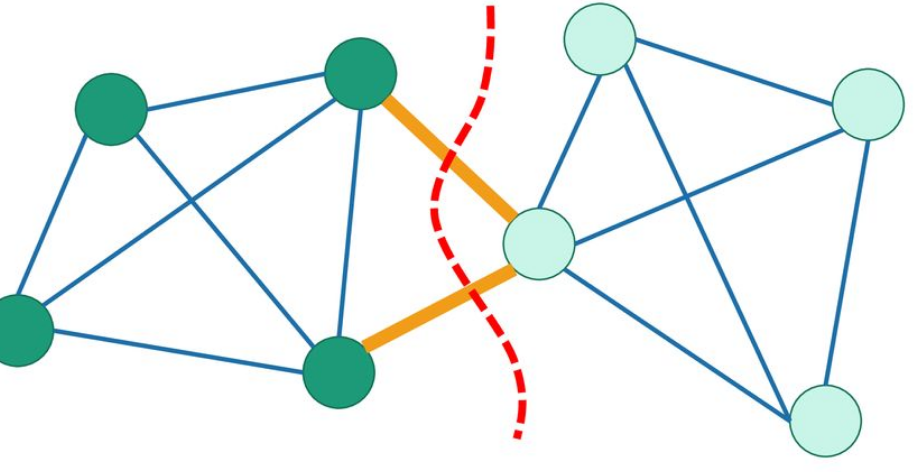
\includegraphics[width=0.8\linewidth]{img/image_2023-01-09-12-40-24.png}
  \caption{Example of global min-cut. Note that the global min-cut is not necessarily unique}
\end{figure}

\marginnote{An example of where this may be useful is in computer networks where we can measure the resiliency of a network by how many cuts must be made before a vertex (or many) get disconnected}


\begin{lemma}
  If the min cut is of size $ \ge k $, then $ G $ is $ k $-edge-connected
\end{lemma}

It may be more convenient to return a set of vertices instead

\begin{definition}
  
\begin{equation}
  S, T \subseteq V, S \cap T = \varnothing 
\end{equation}

\begin{equation}
  E(S,T) = \{(u,v) \in E : u \in S, v \in T\} 
\end{equation}

The global min-cut is to output $ S \subseteq V $ such that $ S \neq \varnothing, S \neq V $,  such that $ E(S, V\setminus S ) $ is minimized.


\end{definition}

\begin{blockquote}

Note that the min-cut-max-flow problem is somewhat of a dual to the global min-cut problem; the min-cut-max-flow problem imposes a few more constraints than the global min-cut algorithm i.e. having a directed and weighted graph as well as the notion of a source or sink.

\begin{itemize}
  \item \textbf{Input: }  Directed, weighted, and connected $ G = (V,E) $, $ s \in V, t \in V $
  \item \textbf{Output}  : $ S $ such that $ s \in S, t \notin S $ such that $  |E(S, V\setminus S ) |  $ is minimized
\end{itemize}
  
\end{blockquote}

We can kind of intuitively see that the global min-cut can be taken to the minimum of all max-flows across the graph.
So we can take the max-flow solution and then reduce it to find the global min cut.

Question: how many times will we have to run max-flow to solve the global min-cut problem? 
Naively, we may fix $ t $ to be an arbitrary node, then try every other $ s \neq t $ to find the $  s-t $ min-cut to get the best global min-cut.

We know from previous courses that the Edmonds-Karp max-flow algorithm will run in $ O(nm^2) = O(n^5) $, which makes our global min-cut algorithm $ O(n^6) $.
However, there is a paper recently published which gives an algorithm for min-cut in nearly linear time, i.e $ O(m^{1-O(1)}) = O(n^2) $  which gives a global min-cut runtime of $ O(n^3) $.

A randomized algorithm will be presented that solves this problem in $ O(n^2 \log^2 n) $


\begin{definition}
  The \textbf{Contraction} operation takes an edge $ e = (u,v) $ and \textit{contracts} it into a new node $ w $ such that all edges connected to $ u,v $ now connect to $ w $ and $ u,v $ are removed. Note that the contracted nodes can be supernodes themselves.

  \begin{figure}[H]
    \centering
    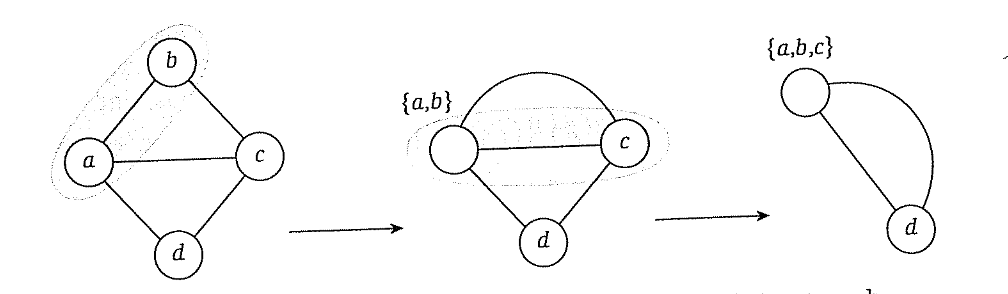
\includegraphics[width=0.8\linewidth]{img/image_2023-01-12-16-47-50.png}
    \caption{Example of a series of contractions}
  \end{figure}

\end{definition}


\begin{codebox}
\Procname{$\proc{contraction}(G=(V,E))$}
\li \While $ G $ has more than 2 supernodes \Do
\li Pick an edge $ e = (u,v) $ uniformly at random
\li Contract $ e $, remove self-loops \End
\li Output the cut $ (S, V \setminus S )$ corresponding to the two super nodes
\end{codebox}

The contraction algorithm then recurses on $ G' $, choosing an edge uniformly at random and then contracting it. 
The algorithm terminates when it reaches \textit{a} $ G' $ with only two supernodes $ v_1, v_2 $. 
The sets of nodes contracted to form each supernode $ S(v_1), S(v_2) $ form a partition of $ V $ and are the cut found by the algorithm.



\subsubsection{Analysis}

The algorithm is still random, so there's a chance that it won't find the real global min-cut.
Perhaps unintuitively the success probability is in fact not exponential, but rather only polynomially small.
Therefore running the contraction algorithm a polynomial number of times can produce a global min-cut with high probability.


\begin{lemma}
  The contraction algorithm returns a global min cut with probability at least $ \frac{1}{\binom{n}{2}} $
  \begin{proof}
    Take a global min-cut $ (A, B) $ of $ G $ and suppose it has size $ k $, i.e. there is a set $ F $ of $ k $ edges with one end in $ A $ and the other in $ B $.
    If an edge in $ F $ gets contracted then a node of $ A$ and a node in $ B $ would get contracted together and then the algorithm would no longer output $ (A, B) $, a global min-cut.
    An upper bound on the probability that an edge in $ F $ is contracted is the ratio of $ k $ to the size of $ E $. A lower bound on the size of $ E $ can be imposed by noting that if any node $ v $ has degree $ < k $ then $ ({v}, V\setminus {v}) $ would form a cut of size less than $ k $ -- which contradicts our first assumption that $ (A,B) $ is a global min-cut; $ |E| \ge \frac{1}{2}kn $
    So the probability than an edge in $ F $ is contracted at any step is

    \begin{equation}
      \frac{k}{(\frac{kn}{2})} = \frac{2}{n}
    \end{equation}

    Note that here we use the number of vertices instead of the number of edges since each contraction removes (combines) one vertex, whereas since the amount of edges after a contraction can be very difficult to calculate.

    Next, let's inspect the algorithm after $ j $ iterations. 
    There will be $ n-j $ supernodes in $ G' $ and we can take that no edge in $ F $ has been contracted yet. 
    Every cut of $ G' $ is a cut of $ G $, so there are at least $ k $ edges incident to every supernode of $ G' $\mn{since the min-cut has $ k $ edges}. Therefore $ G' $ has at least $ \frac{1}{2}k(n-j) $ edges, and so the probability than an edge of $ F $ is contracted in $ j+1 $ is at most
    \marginnote{In terms of edges, it would be $ \frac{k}{m_{i-1}} $, but again, edges are difficult to work with so we'll do it w.r.t the vertices/supernodes}

    \begin{equation}
      \frac{k}{\frac{1}{2}k(n-j)} = \frac{2}{n-j}
    \end{equation}

    It follows that the probability that an edge of $ F $ is \textit{not} contracted in $ j+1 $ is at least

  \begin{equation}
    P(A_i | A_1\ldots_{i-1}) \ge \frac{n-i-1}{n-i+1} = 1 - \frac{2}{n-i+1}
  \end{equation}


  The global min-cut will be actually returned by the algorithm if no edge of $ F $ is contracted in iterations $  1 - n $.

  What we want to know, then, is what is the probability of this algorithm never making a mistake?


  \marginnote{This prof uses commas to indicate intersection...}
  \begin{equation}
    P(A_1 \ldots A_{n-1}) = P(A_1)P(A_2 | A_1) P(A_3 | A_1, A_2) \ldots P(A_{n-2} | A_1, A_2, \ldots, A_{n-3})
  \end{equation}

  From what we found previously we know that this is 

  \begin{equation}
    \ge \frac{n-2}{n} \times \frac{n-3}{n-1} \times \frac{n-4}{n-2} \ldots \times \frac{2}{4} \times \frac{1}{3}  = \frac{2}{n(n-1)} =  \frac{1}{\binom{n}{2}}
  \end{equation}

  \end{proof}

  This gives us a bound of $ O(n^2) $ using the $ n^2 $ term from the number of contractions and then $ n^2 $ to get correct output with constant probability of success.

\end{lemma}


The key observation is that early contractions are much less likely to lead to a mistake, which leads us to the Karger-Stein min cut. 

\subsection{Karger-Stein Min Cut Algorithm}

This algorithm solves the global min-cut problem in $ O(n^2 \log^2 n) $ by taking advantage of the earlier cuts; it stops the contraction algorithm after an arbitrary fraction of contractions steps and then recursively contracts \textit{more carefully}.


\begin{blockquote}

Exercise: show the following:


The probability of no mistake in the first $ i $ contractions
\begin{equation}
  P(A_1, A_2, \ldots A_i) \ge \frac{(n-i)(n-i-1)}{n(n-1)}
\end{equation}
    
\end{blockquote}



\begin{codebox}
\Procname{$\proc{min-cut}(G = (V,E))$}
\li \If $ G $ has two supernodes corresponding to $ S, \hat{S} $ \Then
\li   \Return $ S, \hat{S} $\End 
\li Run the contraction algorithm until $ \frac{n}{\sqrt{2} } + 1 $ supernodes remain
\li Let $ G' $ be the resulting contracted multigraph
\li $ (S_1, \hat{S_1}) = \proc{min-cut}(G') $
\li $ (S_2, \hat{S_2}) = \proc{min-cut}(G') $
\li \Return the cut ($ S_i, \hat{S_i}$) with the smaller number of edges
\end{codebox}

\begin{theorem}
  $ \proc{Min-cut}(G) $ runs in $ O(n^2 \log n) $ and outputs a min cut of $ G $ with probability of at least $ \frac{1}{O(\log n)} $. So we can repeat the algorithm $ O(\log(n)) $ times to get constant probability of success, leading to $ O(n^2 \log^2 n) $ runtime


  \begin{proof}
      The intuition for this can be developed by drawing out a recursion tree for this problem.
      At each level the number of recursive call doubles, but the time it takes for each sub-call halves as well.
      This means that the total runtime for each level is $ n^2 $. 
      As for the total time will just be $ O(n^2 \log (n))$, since we know the height of the recursion tree to be $ \log n $.


      More formally, the recursion may be described with 

      \begin{equation}
          T(n) \le  2T(\frac{n}{\sqrt{2} } + O(n^2))
      \end{equation}

      Which can\mn{I think? } be solved with the master theorem.
      
  \end{proof}
  


\end{theorem}

\begin{theorem}

    We may also want to understand the probability of success. Let's define $ P(d) $ to be the probability of the algorithm being successful at depth $ d $ in the recursion tree\mn{It follows that $ P(h) $ is the probability of the algorithm's success on termination.}

\begin{itemize}
    \item We may deem a node in the recursion tree to be \textit{successful} if it survives the contractions.
        \begin{itemize}
            \item Since there must be a leaf node in a recursion tree that successfully produces a min-cut that corresponds to a min-cut, there must also be a sequence of \textit{successful} nodes from the root to said min cut.
        \end{itemize}
    \item $ P(d) $ as the probability that a node at depth d is successful, conditioned on it's ancestors being successful
\end{itemize}

\begin{itemize}
    \item Base case: $ P(0) \ge \frac{1}{2} $ (will assume $ = \frac{1}{2} $, worst case)
    \item Inductive step: $ P(d) \ge \frac{1}{2} ( 1- (1-(P(d-1)))^2 ) = \frac{1}{2} (2P(d-1) - P(d-1)^2) $ 
      \begin{itemize}
        \item At each level the probability of success is at least $ \frac{1}{2}$, conditioned on the ancestors being successful.
        \item $ P(d-1) $ is the probability of there being a \textit{successful} path from the left child to the root at depth $ d-1 $. The same probability holds for the right sub-child
        \item The two subtrees are disjoint
        \item $ (1 - P(d-1)) $ gives the probability of there \textit{not} being a successful path from a left/right child to the root, $ (1-P(d-1))^2 $ gives the probability that neither of these events hold.
        \item So the probability of success at $ d $ is $ 1 $ minus the prior probability.
      \end{itemize}
\end{itemize}

What remains now is solving this recursion.


\begin{equation}
  P(d) = P(d-1) - \frac{1}{2} P(d-1)^2
\end{equation}

Non-linear recursions are difficult since you really just have to make a good guess. 
It's reasonable to expect this relation to be on the order of 

\begin{equation}
  P(d) \ge  \frac{1}{d}
\end{equation}

And then as it turns out\mn{Proof by trust-the-prof} it's 

\begin{equation}
  P(d) = \frac{1}{d+2}
\end{equation}

And then this can be checked by doing an induction proof, but I'm not going to go and do that.

\end{theorem}


\marginnote{

  Note that there are two types of randomized algorithms:

  \begin{itemize}
    \item Monte Carlo algorithms: bound on worst-case time \& produces a correct answer with a probability $ \ge  $ some constant
    \item Las Vegas algorithms: bound on the expected value of running time, but the output is always correct
  \end{itemize}
  Our contraction algorithm is a Monte-Carlo algorithm
}


\subsection{Closest Pair Problem}

The closest pair problem is simple: given the \textbf{Input}: A set $ P $ of $ n $ points in the plane, find the \textbf{Output}: A pair of points $ p, q \in P $ such that $ d(p,q) $ (some distance metric, often euclidean or hamming distance) is minimized.


We are already familiar with a few approaches:

\begin{itemize}
    \item Brute force: $ O(n^2) $
    \item Divide and conquer (CLRS 33.4): $ O(n\log n) $
\end{itemize}


A tighter linear time bound may, remarkably, be achieved through a randomized algorithm and a slightly different approach to hashing than what we are used to.


\begin{codebox}
\Procname{$\proc{rabins-algorithm}(P)$}
\li Randomly order $ P $ as $ p_1, p_2 \ldots p_n $
\li $ cp = \{p_1, p_2\} $
\li $\Delta = dist(p_1, p_2)$
\li \For $ i = 3 $ to $ n $ \Do
\li     \If $ \exists q \in P_{i-1} = {p_1 \ldots p_{i-1}} \text{ s.t. }dist(p, q) < \Delta $ \Then
\li     $ cp = \{p, q\} $
\li     $ \Delta = dist(p, q) $ \End \End
\end{codebox}

Rabin's algorithm considers the points in random order, maintaining a current minimum pair distance $ \delta $ as points are processed. At every point $ p $ we look in the \textit{vicinity} of $ p $ to see if any of the previously considered points are within $ \delta $ from $ p $, i.e. will form a closer pair.
The tricky part of this algorithm is performing the \textit{check\_closest} operation in constant time.

Considerations to make:

\begin{itemize}
    \item It is possible to randomly order $ P $ from $ n! $ possible orderings in $ O(n) $ time (CLRS reference for later)
    \item What data structure to use for line 5? I.e. finding $ q $ such that $ dist(p, q) < \Delta $
        \begin{itemize}
            \item Note: take $ q $ that is closest to $ p_i $ in line 5 (algorithm is unclear as to pick $ p_1 $ or $ p_2 $)
            \item This data structure must store a set $ Q = P_{i-1} = {p_1, p_2, p_{i-1}} $ points and offer the following operations
            \begin{itemize}
                \item Note: $ \Delta(Q) = \delta = min_{p, q \in Q, p \neq  q} dist(p,q)  $
                \item $ \proc{insert-fast}(p) $ inserts $ p $ into $ Q $ assuming $ min \left\{  dist(p,q) : q \in Q \right\} \ge  \delta $
                \item $ \proc{insert-slow}(p) $ inserts $ p $ into $ Q $ even if $ min \left\{  dist(p,q) : q \in Q \right\} <  \delta $
            \item $ \proc{check-closest}(p) $ checks if $ min \left\{  dist(p,q) : q \in Q \right\} < \Delta $ and if so returns the closest point $ q  \in Q$ to $ P $, otherwise returns $ NIL $. Runs in $ O(1)  $ expected time
            \end{itemize}
        \end{itemize}
\end{itemize}

Here the, well, structure, of the data structure begins to become apparent.
By making the assumption that the smallest distance so far is $ \delta $ we can perform the requisite lookup/insertions in constant time (only need to look in a ring of size $ \delta $ around $ p $) -- and if we do happen to find a yet-closer pair of points then some modification would have to be made to maintain the $ \delta $ invariant.

Here's Rabin's algorithm in more detail:
\begin{codebox}
\Procname{$\proc{rabins-algorithm}(P)$}
\li Randomly order $ P $ as $ p_1, p_2 \ldots p_n $
\li $ cp = \{p_1, p_2\} $
\li $\Delta = dist(p_1, p_2)$
\li Initialize the data structure with $ \left\{  \right\}  $
\li \For $ i = 3 $ to $ n $ \Do
\li    $ q = \proc{check-closest}(p_1) $
\li    \If $ q == NIL$ \Then
\li        $ \proc{insert-fast}(p_i) $
\li    \Else
\li        $ cp = \left\{ p_1, q \right\}  $
\li        $ \Delta = dist(p_1, q) $
\li        $ \proc{insert-slow}(p_1) $ \End \End
\end{codebox}

It's fairly trivial to see that this algorithm has a $ O(n^2) $ worst case runtime;
Line 1 is $ O(n) $, and all the inserts run in $ O(1) $ expected. In the worst case event that we would $ \proc{insert-slow} $ which would cause the runtime to tend towards $ O(n^2) $. 
It is our job now to find out just how often this would happen, and as it turns out it really isn't altogether that often -- leading to an $ O(n) $ runtime.
Before that, however, we still need to formalize the data structure that enables this black magick? \textbf{Idea: } draw grid with side length $ \frac{\delta}{2} $.
If a point $ q $ being inserted belongs to the same sub-square $ S_{st} $ as $ p $, then $ d(p, q) < \delta $. 
If we take $ Q $ to be the set of points currently in the data structure, then since

\begin{equation}
    \frac{\delta}{\sqrt{2} } < \delta
\end{equation}
No two points in $ Q $ fall within the same square.

A partial converse is also true: If a point $ q $ being inserted that gives $ dist(p, q) \le  \delta $ than each other must fall in either the same subsquare or in very close subsquares.


\begin{figure}[H]
\centering
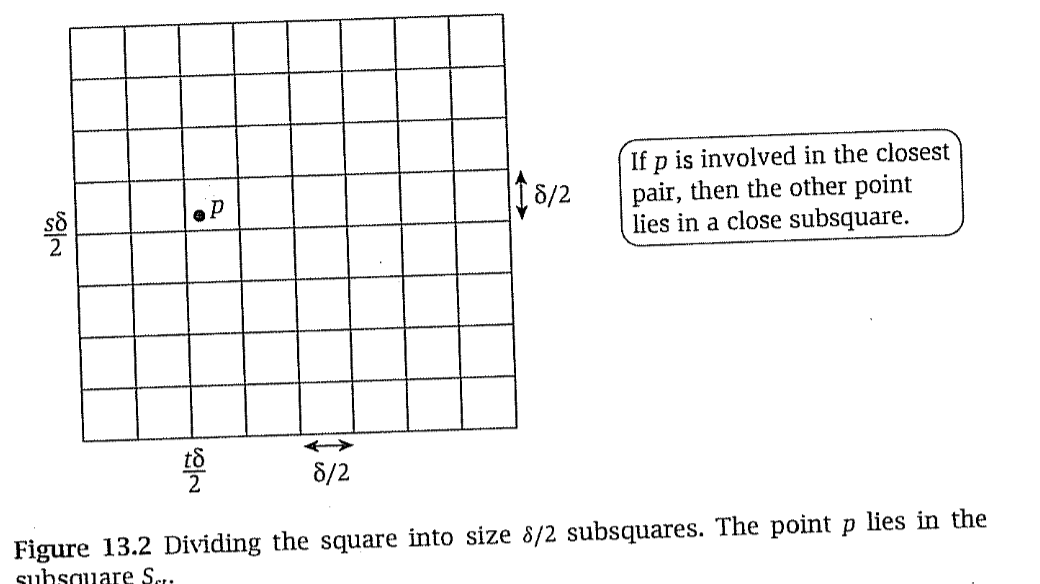
\includegraphics[width=0.8\linewidth]{img/image_2023-01-20-12-40-20.png}
\end{figure}

Implementation-wise we require a data structure with fast lookup of these subsquares. A natural data structure for this is a dictionary. 

As for the key we use to index into the dictionary -- this will depend on the specific space across which we are finding the closest points.
For floating point Cartesian coordinates we may use use the floor function.

\begin{itemize}
    \item Insert-fast: just insert into the dictionary
    \item Insert-slow: must do the rather dramatic operation of rebuilding the data structure with new $ \delta$, since the old data structure is now entirely invalidated.
    \item Check-closest: Must look in the 25 squares around $ p $ for points closer than $ \delta $. If there are more just return the closest. \mn{Note that we have to search the 25 squares around $ p $ since $ p $ may be located anywhere within the grid cell. In the worst-case situation it lies on the edge of a grid cell and therefore we must search up to two sub-squares away.}
\end{itemize}

\subsubsection{Analysis}

\begin{itemize}
    \item Recall $ P_i = \left\{ p_1 \ldots p_i \right\}  $. Define (for $ i \ge  3 $) $ Z_i = 
        \begin{cases}
            1 & \Delta(P_i) < \Delta(P_{i-1}) \\
            0 & \text{ otherwise}
        \end{cases} $ 

        \begin{itemize}
            \item This is a random event since the order of points is random. The first case represents a slow insert and the other a fast insert. If we take $ Z_i $ denote the probability of a slow insert, then the runtime of the algorithm is given by:
                \begin{itemize}
                    \item $ T \le n + \sum_{i=3}^{n}(1 + i Z_i) $ 
                    \item $ n $ for the random init, $ 1 $ for fast insert and $ iZ_i $ for a slow insert
                \end{itemize}
            \item We are primarily interested in the expected value of $ T $, not the worst-case runtime.

                \begin{equation}
                    \begin{split}
                        E[T] & \le n + (n-2) + \sum_{i+3}^n i \cdot EZ_i \text{  by linearity of expectation} \\
                         & = 2n-2 + \sum^n_{i=3} i \cdot  P(Z_i = 1) 
                    \end{split}
                \end{equation}
        \end{itemize}
    \item Now, what's $ P(Z_i) = 1 $?
        \begin{itemize}
            \item Let $ \left\{ p_i, p_k \right\} $ be a closest pair in $ P_i $
            \item If $ Z_i  = 1$  then $ p_i $ or $ p_k $ is $ p_i $
            \item $ P(Z_i = 1) \le  \frac{2}{i}  $ (There are two bad options out of i options)
        \end{itemize}
    \item By combining the above two results we can obtain the following bound on the algorithm running cost

        \begin{equation}
            E[T] \le  2n-2 + \sum^n_{i=3} i \cdot  P(Z_i = 1) = 2n-2 + \sum^n_{i=3} i \cdot \frac{2}{i} \le  O(n)
        \end{equation}
\end{itemize}


\subsection{Tutorial: Locality Sensitive Functions}

\begin{blockquote}
    \begin{figure}[H]
        \centering
        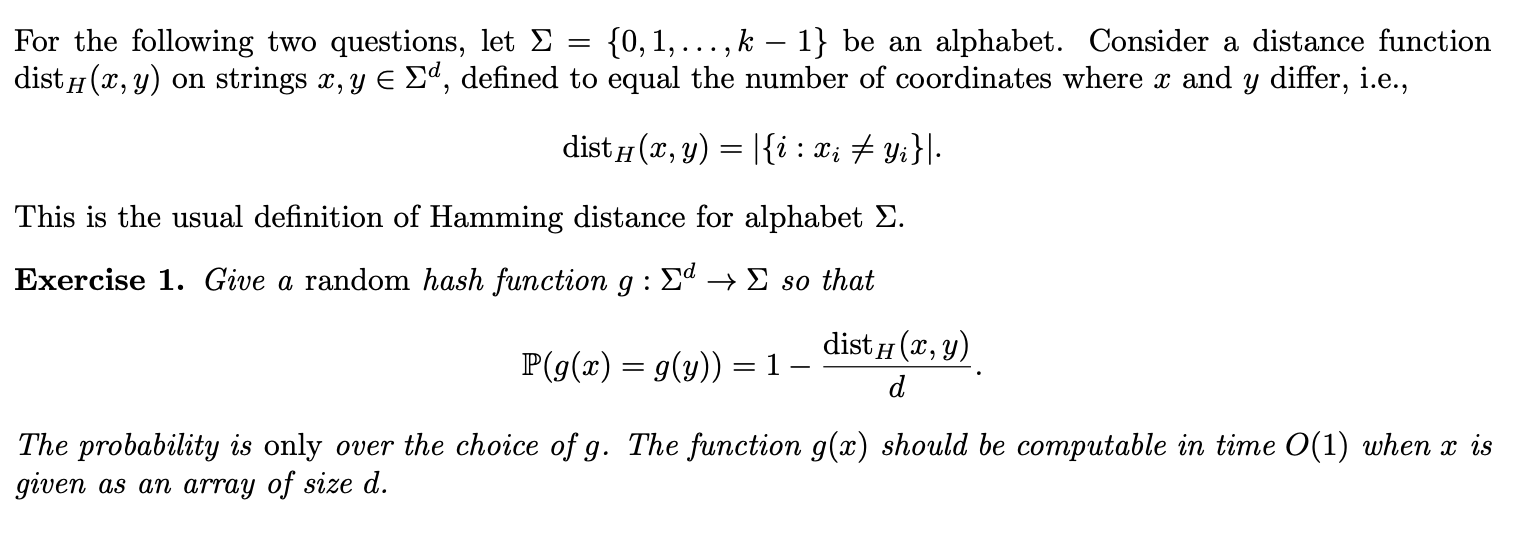
\includegraphics[width=0.8\linewidth]{img/image_2023-01-25-12-12-15.png}
        \caption{Q1}
    \end{figure}
\end{blockquote}


Randomly sample a dimension\mn{O(1)} and then the probability of the hash functions being equal to each other is proportional to the hamming distance between the strings (consider random...).

\begin{figure}[H]
    \centering
    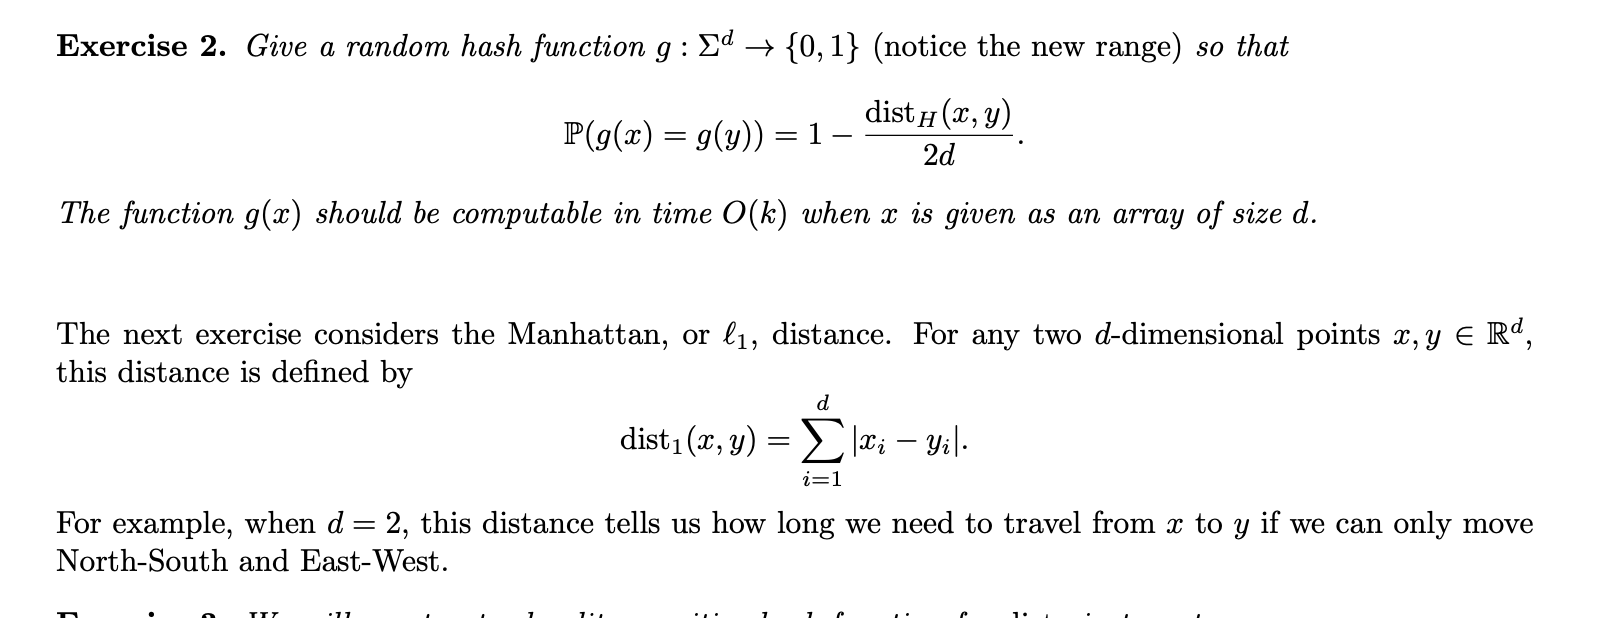
\includegraphics[width=0.8\linewidth]{img/image_2023-01-25-12-39-13.png}
    \caption{Q2}
\end{figure}


\begin{enumerate}
    \item Sample a dimension $ d $ uniformly at random
    \item In that dimension, assign each letter on $ k-1 $ to $ \left\{ 0, 1 \right\}  $uniformly at random
\end{enumerate}


P(equal) is 1-  sum not equal / 2 = hamming dist / 2 * d (d letters)

This works because $ P(g(x) \neq  g(y) | \text{selected dimension i}) = \frac{|\left\{ i x_i \neq  y_i \right\} }{2d} $.


O(k) since you have to sample it k times



\begin{figure}[H]
    \centering
    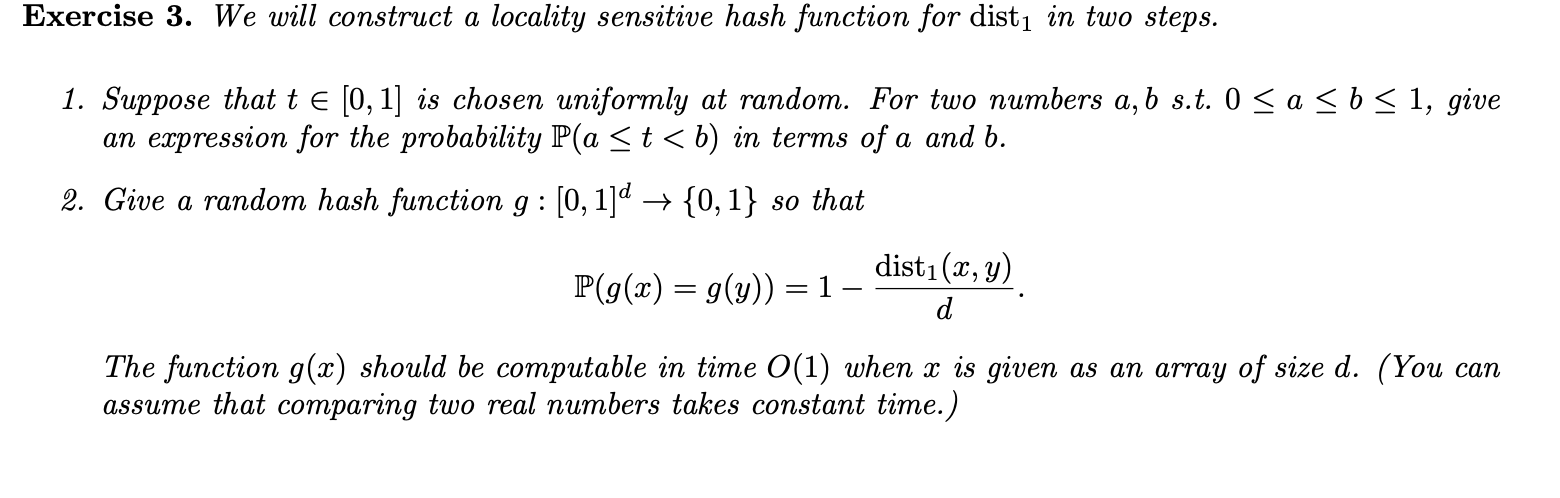
\includegraphics[width=0.8\linewidth]{img/image_2023-01-25-12-39-25.png}
    \caption{Q3}
\end{figure}

\begin{blockquote}
    I honestly don't really know how this one works :(
\end{blockquote}


\begin{itemize}
    \item pick a dimension at random
    \item Sample a $ t \in (0, 1) $ uniformly at random
    \item if the value smaller than t -> 0, larger than t -> 1
    \item P(g(x) != g(y) | selected dim i+ = |x\_i - y\_i
    \item given $ 0 \le  a \le  b \le  1 $, $ P(a \le  t < b) $  is 
\end{itemize}

\subsection{Nearest Neighbours \& Clustering}

Suppose we have a data set $ P $ of $ n $ entries\mn{which usually are points in some metric space, i.e. a space that is reflexive, symmetric, and satisfies the triangle inequality}, how may we design a data structure that can efficiently output a point $ y \in P $ that has the smallest distance $ dist(x,y) $ to $ x $?

\subsubsection{Hamming Distance}

\begin{definition}
    \textbf{Hamming Distance}: number of bits that differ between two strings

    \begin{equation}
        dist(x,y) = |\left\{ i : x_i \neq  y_i \right\} |
    \end{equation}


    
\end{definition}

Let there be a data set $ P $ containing $ n $ strings with $ d $ bits each, i.e. $ P $ is a subset of $ \left\{ 0, 1 \right\} ^d $. 

We want our data structure to support the following operations:

\begin{itemize}
    \item $ \proc{insert}(P, x) $: insert $ x $ into $ P $
    \item $ \proc{nearestneighbour}(P, x) $: output the closest $ y $ to $ x $ in $ P $
\end{itemize}

\marginnote{Exercise: Give a data structure for which we have $ O(1) $ insert and $ O(2^d) $ lookup}

As it turns out this problem is nontrivial; this problem suffers from the \textit{curse of dimensionality}. 

We can relax the time bounds by relaxing the constraints on the problem somewhat to the approximate nearest neighbour problem

\begin{definition}
    $ \proc{ApxNearestNeighbour}(P, x) $: output a string $ y \in P $ such that 

    \begin{equation}
        min \left\{ dist(x, z) : x \in P \right\}  \le  dist(x, y) \le  C \cdot  min \left\{ dist(x, z) : z \in P \right\} 
    \end{equation}

    I.e. we do not need to find the exact nearest neighbour and are satisfied with a neighbour that is good enough (within an approximation factor $ C $) of the nearest neighbour.

\end{definition}

Indyk and Motwani propose a clever hashing scheme for a randomized data structure to solve this problem in $ O(dn^p) $ time where $ p \approx \frac{1}{C} $ and $ \proc{ApxNearestNeighbour}(P, x) $ will output a C-near neighbour with probability at least $ \frac{2}{3} $ via a new function, $ \proc{NearNeighbour}(P, x) $


\begin{definition}
    $ \proc{NearNeighbour}_r(P, x) $
    \begin{itemize}
        \item If $ \exists z \in P  $  such that $ dist(x, z) \le  r $, then $ \proc{NearNeighbour}_r(P, x) $  will output some $ y \in P $ for which $ dist(x,y) \le  Cr $
        \item If every string $ z $ in $ P $ satisfies $ dist(x, z) \ge  Cr $, then $ \proc{NearNighbour}_r(P, x) $ outputs FAIL.
    \end{itemize}
\end{definition}


Next, let's go from $ NearNeighbour $ to a harder problem: $ \proc{NearestNeighbour}(P, q) $ via $ \proc{ApxNearestNeighbour}(P, q) $

\begin{itemize}
    \item  Assume that for each $ r $ we can implement a data structure for an easier problem (e.g. $ \proc{NearNeighbour}(P, q) $) for which $ \proc{Insert}, \proc{NearNeighbour}$ run in $ T(n) $, how can we implement Insert and ApxNearestNeighbour in $ O(T(n)\log d) $ so that $ \proc{ApxNearestNeighbour} $ achieves approximation factor $ 2C $ and success probability $ \frac{2}{3} $
\end{itemize}


How can we build this data structure then? \marginnote{Still focusing on hamming distance for now}

\begin{itemize}
    \item Looking at euclidean distance, what if we divide $ \mathbb{R}^d $ into grid cells and then $ \proc{NearNighbour}(P, q)$ checks the cells around $ q $. This won't work because the amount of cells we have to check is an exponential in the order of $ d $.\mn{This is particularly an issue with hamming distance since here we commonly work with very high dimensions. Not as bad for euclidean distance since usu. work with 2-3 dimensions there.}
    \item We can cut down on the number of cells we have to check by forming the cells randomly. This way, though we introduce the possibility of making a mistake, we also greatly reduce the number of cells to check.
\end{itemize}


Instead of a fixed grid we randomly divide the string $ \left\{ 0, 1 \right\} ^d $ into buckets such that
\begin{itemize}
    \item $ dist(x,y) \le  r \Rightarrow  (x,y )$  fall into the same bucket with probability $ \ge p_1 $
    \item $ dist(x,y) \ge Cr \Rightarrow  (x,y )$  fall into the same bucket with probability $ \ge p_2 $
\end{itemize}

and $ p_1 > p_2 $.

Taking a step back the idea is that we can create buckets and hash into the bucket in such a way that it is more likely for near neighbours of $ x $ to fall in the same bucket of $ x $ and likewise for strings far from $ x $. 
After the strings have been separated off into buckets the specific near neighbours can be found through normal hashing\mn{or whatever you choose at this point, I think}. $ \proc{NearNeighbour}(P, q)  $ checks the bucket containing $ q $ and repeats the whole thing several times.

Now, how can we do this for hamming distance?

\begin{definition}
    For any $ i \in \left[ d \right], g_i : \left\{ 0, 1\right\}^d \to \left\{ 0, 1 \right\} $ is defined by $ g_i = x_i $.
    Suppose $ i $ is picked from $ \left[ d \right] $ uniformly at random.\mn{Instead of thinking hash functions we can also think of this as the buckets we are putting values in (or are getting hashed to)}
    Then the probability of a hash function collision is:

    \begin{equation}
        \mathbb{P}_i(g_i(x) = g_i(y) ) = \frac{\left\{ i: x_i = y_i \right\} }{d} = 1 - \frac{\left\{ i: x_i \neq  y_i \right\} }{d} = 1- \frac{dist(x,y)}{d}
    \end{equation}

    Where $ dist $ is the hamming distance between $ x, y $
\end{definition}

Then, the probability that they are mapped to the same value, i.e. that near points collide is:

\begin{equation}
    dist(x,y) \le  r : P(g_i(x) = g_i(y)) \ge (1 - \frac{r}{d})^k = p_1^k
\end{equation}

And that they don't collide:

\begin{equation}
    dist(x,y) \ge  Cr : P(g_i(x) = g_i(y)) \le  (1 - \frac{Cr}{d})^k = p_2^k
\end{equation}


This is a locality-sensitive hashing family for hamming distance. 
In this case it is quite similar for the hamming distance case, but it can be more difficult for different distances.
Unlike other hashing functions the probability of collision is not constant, but depends on the distance between the points.


We may amplify the probability gap by hashing multiple times. This is a very generic technique that applies to other distance metrics and hashing methods as well.

\begin{definition}
    For $ I = (i_1 \ldots i_k) $ a sequence of indicies from $ \left[ d \right], g_j  $  is defined by $ g_I = (x_{i_1}, \ldots x_{i_k}) $.


    For $ I = (i_1 \ldots i_k) $ picked uniformly and independently from $ \left[ d \right]  $,

    \begin{equation}
        \begin{split}
        \mathbb{P}(g_I(x) &=  g_I(y) ) = P(x_{i_1} = y_{i_1}, \ldots x_{i_k} = y_{i_k})  \\
        &= P(x_{i_1} = y_{i_1}) \ldots P(x_{i_k} = y_{i_{k}}) \\
        &=  1 - \left( \frac{dist(x,y)}{d} \right)^k  
        \end{split}
    \end{equation}

    So,

    \begin{equation}
        dist(x,y) \le  r : P(g_I(x) = g_I(y)) \ge 1 - \left( \frac{r}{d} \right)^k = p_1^k
    \end{equation}

    \begin{equation}
        dist(x,y) \ge  Cr : P(g_I(x) = g_I(y)) \le  1 - \left( \frac{Cr}{d} \right)^k = p_2^k
    \end{equation}

    So this gives us the power to pick $ k $ arbitrarily in order to amplify the gap between $ p_1 $ and $ p_2 $
    \begin{itemize}
        \item $ k $ is a parameter that we will choose.
    \end{itemize}

    \begin{example}
        $ x = (1,0,0,0,1,1,1,0) $, $ I = (3,1,7) $
        \begin{equation}
            g_I(x) = (0,1,0)
        \end{equation}
        
    \end{example}
    

\end{definition}

\subsubsection{Two-level hashing}

Data structure:

        \marginnote{
            Note: universal hash functions are hash functions such that
            each $ h_i $ is a random hash function that such that 
            \begin{equation}
                \forall u, v \gets \left\{ 0, 1 \right\}  ^k, u \neq v  
            \end{equation}

            The probability of collision for an universal hash function is small, or formally,

            \begin{equation}
                P(h_i(u) = h_i(v)) \le \frac{1}{m} \le  \frac{1}{n}
            \end{equation}

            TLDR: has a reasonably low probability of collision and is reasonably fast to compute
        }

        \begin{itemize}
            \item $ L $ hash tables $ T_1 \ldots T_L $ with $ m \ge  n $ slots each
            \item L regular hash functions $ h_1 \ldots h_L : \left\{ 0, 1 \right\}^k \to \left[ m \right] $ from an universal family
            \item  L locality sensitive hash functions $ g_{I_1} \ldots g_{I_l} : \left\{ 0, 1 \right\} ^d \left\{ 0, 1 \right\} ^k$
\end{itemize}


\textbf{Structure and inserting}

Store each $ x \in P $ in $ T_l[h_l(g_{I_l}(x))], l = 1 \ldots L $.
\begin{itemize}
    \item $ g $ is the locality sensitive hash function and $ h $ is the regular hash function.
    \item $ g $ is used to map the point into buckets which are `close together' and then $ h $ is used to resolve locally clustered points. Collisions can be handled via linear chaining.
    \item runtime on the order of $ O(lp) $ for insertion
\end{itemize}

\begin{codebox}
\Procname{$\proc{nearneighbour}(P, q)$}
\li $\text{num-checked} = 0$
\li \For $ l \gets 1 $ \To L \Do
\li     $ i = h_l(g_l(q)) $
\li     set $ x $ to the head of $ T_l[i] $
\li     \While $ x \neq \varnothing $  \Do
\li         \If $ dist(q.x) <= Cr $ \Then 
\li             \Return $ x $ \End
\li         $\text{num-checked} = \text{num-checked} + 1$
\li         \If $ \text{num-checked} = 12L + 1$ \Comment{timeout} \Then
\li             \Return FAIL \End
\li         \Else
\li             Set x to the next element in $ T_l[i] $ \End \End \End
\li \Return FAIL
\end{codebox}

In words: for each hash table $ T_l $ search through $ T(h_l(g_l(x))) $ linked list. If we find a near neighbour, we're good. Otherwise, keep on trying until we timeout (Line 9) (just some somewhat arbitrary constant) or fail otherwise.


\begin{definition}
    \textbf{Union Bound} 

    For any two events $ A, B $ in a probability space ,

    \begin{equation}
        P(A \text{ or } B) \le   P(A) + P(B) 
    \end{equation}

    And by simple induction this extends to $ k $ events
\end{definition}



\textbf{Analysis} 

Or goal here is to show that the probability of `bad collisions' or failure is small.

\begin{theorem}

    Let $ k = \log_{\frac{1}{p_2}}(n)$. Let $ \rho = \frac{\log \frac{1}{p_1}}{\log \frac{1}{p_2}} $ and $ L = 2n^{\rho} $. 
    If there exists a point  $ x^* $ in $ P $ such that $ dist(x, x^*) \le r  $, then with probability of at least $ \frac{2}{3} $ the procedure $ \proc{nearneighbour}(P, x) $ will output some $ y \in P $ for which $ dist(x,y) \le Cr $

\end{theorem}

We assume that there exists $ x^* \in P  $ such that $ dist(q, x^*) \le r $, i.e. there is some point $ x^* $ in the dataset that is somewhat close to $ q $.
Therefore there exists a circle of radius $ Cr $ centered about $ q $ containing all of the points that could satisfy $ \proc{nearneighbour} $

Conversely we can produce the set $ F $ of far-away points as follows

\begin{equation}
    F = \left\{ x \in P: dist(q, x) > Cr \right\} 
\end{equation}


$ \proc{NearNeighbour}(P, x) $ succeeds if it outputs some $ y \in P  $ such that $ dist(x,y) \le  Cr $. For this to happen we must have:

\begin{enumerate}
    \item $ q $ collides with points in $ F $ at most $  12L $  times (with multiplicity)
    \item $ q $ collides with $ x^* $
\end{enumerate}

\marginnote{It's really difficult to do this proof with a statement like `probability of hitting 12L+1 consecutive items in $ F $' since that implies an ordering.}


What is the probability of both happening?


\begin{enumerate}
    \item \textbf{Expected number of collisions with far points}


\begin{blockquote}
    Recall that $ p_2 = 1 - \frac{Cr}{d} $ is the probability that near points do not collide.
\end{blockquote}

\begin{equation}
    \forall l, \forall x \in F: P[g_{I_l}(x) = g_{I_l}(q)] \le  p_2^k = (1-\frac{Cr}{d})^k
\end{equation}

\marginnote{I.e. the probability of a collision with a far away point is bounded by the probability that near points do not collide}

Let us choose $ k  $ such that

\begin{equation}
    p_2^k = (1-\frac{Cr}{d})^k \le  \frac{1}{n} \Rightarrow k \equiv \frac{\log n}{\log \frac{1}{p_2}}
\end{equation}


Let's define a random indicator variable $ z_{x, l} $ which takes on $ 1 $ if $ y $ collides with $ x $ in $ T_l $ and $ 0 $ otherwise.
The number of collisions with far points is then the expectation of this random variable.

\begin{equation}
    z_{x,l} =
    \begin{cases}
        1 & \text{if x collides with q in T\_l} \\
        0 & \text{otherwise}
    \end{cases}
\end{equation}

\begin{equation}
    E[X] = \sum^L_{l=1} \sum_{x \in F} z_{x,l} \le  \frac{2|F| L}{n} \le 2L
\end{equation}

\sidenote{Since we defined $ F $ to be the set of far collisions and $ |F| $ is just the number of items in $ F $. }

\begin{definition}
    \textbf{Markov's Inequality} 

    Let $ X \ge 0 $ be a random variable. Then for any $ x > 0$,

    \begin{equation}
        P(X > x) < \frac{E[X]}{x}
    \end{equation}

    \begin{proof}

    By the law of total expectation we can break up the expectation into two parts

    \begin{equation}
        E[X] = E[X | X\le x] \cdot P(X \le x) + E[X | X > x] P(X>x)
    \end{equation}

    The first term is non-negative and the 2nd term is strictly larger than $ xP(X > x) $. So 

    \begin{equation}
        E[X] > x P (X > x)
    \end{equation}
    \end{proof}

    Note that a similar result holds for

    \begin{equation}
        P(X \ge x) \le  \frac{E[X]}{x}
    \end{equation}

\end{definition}


We will also need to know how an element $ y $ can collide with $ q $ in $ T_l $.
A string $ y $ will collide with $ q $ if $ h_l(g_{I_L}(y)) = h_l(g_{I_L}(x)) $ for some $ l $.
This implies that that collisions happen if

\begin{enumerate}
    \item $ g $ produces the same output for $ y $ and $ q $ for some $ l $, i.e the first hash function collides
    \item $ h_l $ produces the same output for different inputs\mn{Those being the result of the first hash function}, i.e. $ h $ collides
\end{enumerate}

Since we picked each hash table to have $ m \ge  n $ slots and that $ h_l $ is chosen from a family of universal hash functions, we have the probability of $ h $ colliding being bound by $ \frac{1}{n} $. 
For $ g $ we picked $ k $ carefully a little bit prior such that the probability of collision is bounded by $ p_2^k \le  \frac{1}{n}$

Therefore we have

\begin{equation}
    \begin{split}
        P[z_{x,l} = 1] &= P[g_{I_l}(x) = g_{I_l}(q)] + P[g_{I_l}(x) \neq g_{I_l}(q), h_l(g_{I_l}(x))  \\
&=  h_l(g_{I_l}(q))] \le  \frac{1}{n} + \frac{1}{n} \le  \frac{2}{n}
    \end{split}
\end{equation}

\sidenote{Note that the probability of collision is at most $ \frac{1}{n} $ for an universal hashing function}

Then we can apply Markov's inequality to get that the probability of the random variable $ Z $ representing the number of collisions as

\begin{equation}
    P[Z \ge  12L] \le  \frac{2L}{12L} = \frac{1}{6}
\end{equation}

So this property holds with probability of at least $ \frac{5}{6} $

\marginnote{This implies that a relationship between Monte Carlo and Las Vegas algorithms; we can take a Las Vegas algorithm and turn it into a Monte Carlo algorithm by timing it out.}

\item  \textbf{Now we have to show the probability of $ q $ collides with $ x^* $ or \textit{something good}}

For the proof we'll take $ x^* $ since we assumed it to be good earlier on.

This probability is lower-bounded by the probability that there exists a $ l $ such that $ g_l $ produces the same output for $ x^* $ and $ q $.
However we want to bring on a upper bound to this probability.


\begin{equation}
    \begin{split}
        P(\exists l : g_{I_l}(q) = g_{I_l}(x^*)) &= 1-\prod^L_{l=1} P[g_{I_l}(x*) =  g_{I_l}(q)]  \\
        &\ge 1 - (1-p_1^k)^L \ge  1 - e^{-L p_1^k} 
    \end{split}
\end{equation}


\begin{blockquote}
    Recall: $ p_1 = 1 - \frac{r}{d} $  is the probability of a collision with a near point i.e. $ dist(x,y) \le r $

    Also, it's a fact that $ 1-x \le  e^{-x} $
\end{blockquote}


Then we can simplify this a little bit by assuming $ k = \log_{\frac{1}{p_1}} n $

\begin{equation}
    p_1^k = 2^{-k \log_2 (\frac{1}{p_1})} = \ldots n^{-\rho}
\end{equation}

So then we have $ Lp_1^k = 2 $ and $ x^*  $ collides with $ x $ with probability at least $ 1-\frac{1}{e^2} $.


\end{enumerate}

By the union bound bound the probability of both properties holding is at least


\begin{equation}
    1 - (\frac{1}{6} + \frac{1}{e^2}) > \frac{2}{3}
\end{equation}

which concludes the proof.


This also implies that $ \proc{INSERT}, \proc{nearneighbour} $ run in $ O((k+d)n^{\rho}) $ (Recall: $ k $ is the input string size, $ d $ is the number of buckets, and $ L \approx n^\rho$).
Approximating $ 1 -x \approx e^{-x} $ we get $ \rho = \frac{\log \frac{1}{p_1}}{\log \frac{1}{p_2}} \approx \frac{1}{C} $ and $ k = O(d\log(n)) $. 
So overall they run in approximately $ O(dn^{\frac{1}{C}} \log n) $ time which is much faster than $ \Theta(dn) $ linear search for $ C > 1 $




Now we may be interested in extending what we have done for Hamming distance for other distance metrics, i.e. having a hash function that is more likely to put nearby points in the same bucket than far away points.



\begin{definition}
    A random hash function $ h $ with domain $ X $ is \textit{locality sensitive} with parameter $ p $ for distance metric $ d $ if

    \begin{equation}
        dist(x, y) \le  r \Rightarrow P(h(x) = h(y)) \ge  p_1
    \end{equation}

    \begin{equation}
        dist(x, y) \ge   Cr \Rightarrow P(h(x) = h(y)) \le  p_2
    \end{equation}
    


\end{definition}



\subsection{Streaming Algorithms}

Streaming algorithms are a class of algorithms that are extremely efficient in terms of space and usually in terms of time complexity.
They are used in many applications where we want to process enormous amounts of data in a short amount of time.
Generally they are algorithms that work in time steps and receive one update per time step.


Here are some definitions and conventions for the following section


\begin{itemize}
    \item The sequence of updates is called the \textit{stream}
    \item $ n $: the size of the universe the stream is coming from
    \item $ m $: the length of the stream (may/may not be given to algorithm)
    \item Algorithm is only allowed to store a number of bits which is bounded by a polynomial in $ \log n $ and $ \log m $, i.e. $ O(\log^c (nm)) $ bits.
\end{itemize}

Many fundamental streaming problems are summarized by the frequency vector $ f $ which describes the number of times each element in the universe appears in the stream.\mn{The algorithm cannot actually store $ f $ since it's size is $ O(n) $ which violates the memory bound described earlier}

Some other versions of the streaming model may introduce a richer meaning to update, i..e the \textit{turnstile} model where an update is a pair $ (i,s) $ where $ i $ identifies the update and $ s $ identifies the type of update it is\mn{For example entering or exiting a subway station}



\begin{example}
    \textbf{Give an algorithm that finds the missing number in a stream of $ n-1 $ numbers containing $ n-1 $ of the integers $ 1 \ldots n $}

    This can be solved by taking the running sum of the stream and subtracting it from the sum of numbers from $ 1 \ldots n $. 
    A likewise approach may be adopted to $ 2 $ missing numbers by introducing the sum of squares.
\end{example}



\subsubsection{Frequent Elements}

As a warm-up let's consider the majority problem

\begin{itemize}
    \item \textbf{input: } a stream $ \sigma = (i_1 \ldots i_m) $ of updates in $ [n] = {1....n} $.
        If there exists $ i \in [n] $ such that more than half of the updates in $ \sigma $ are equal to $ i $, the algorithm should output $ i $. Otherwise, it may output any element
\end{itemize}

The following algorithm proposed by Boyer and Moore solves the problem with only two words of memory

\begin{codebox}
\Procname{$\proc{MAJORITY}(\sigma)$}
\li $ element = i_1 $
\li $ count = 1 $
\li \For $ t \gets 2 \To m $ \Do
\li \If $ element == i_t$ \Then
\li     $count = count + 1 $
\li \ElseIf $ count > 0 $ \Then
\li     $ count = count - 1 $
\li \Else
\li     $ element = i_t $
\li     $ count = 1 $ \End \End
\li \Return $ element $
\end{codebox}

\begin{proof}

    A naive implementation of a solution could involve storing $ f $, i.e pairs of each unique element and it's associated frequency.
    However this uses a lot more space than what we desire. 
    We note that for this problem we don't care about the actual frequency of each element, only the element with the highest frequency, so the problem solution may be relaxed to only store the element [with the highest frequency]. 
    Likewise, we don't care about the frequency of the element either -- only that it is the highest frequency element.
    The above algorithm maintains the invariant that $ f_{element} \le count + \frac{m}{2}$.

    Therefore by the time the algorithm finishes executing $ element $ will contain the most frequent element (if there exists one) or some arbitrary element otherwise.
    Intuitively we may think of the procedure "allocating" space for one non-current-majority element on lines 4-5, which can then be taken away if we later inspect a non-current-majority element (lines 6-7).
    Then it can be concluded that if an element `survives' until the end of the algorithm it must either 1. be the majority element, if one exists, or 2. any arbitrary element, if none exists.

    
    \begin{blockquote}
    Note that Since this algorithm does not tell you if a strict majority exists or not, to verify it's results you will have to run over the data set again to determine if the resulting value is the majority value or just \textit{any} element.
    \end{blockquote}
    
\end{proof}


An extension of $ \proc{Majority} $ is given by Misra and Gries to find all elements that appear in more than $ \frac{1}{k} $ of the updates


\begin{codebox}
\Procname{$\proc{frequent}(\sigma, k)$}
\li $ S = \emptyset $
\li \For $ t \gets 1 \to m $ \Do
\li     \If $ \exists x \in S  $ such that $ x.elem == i_t $ \Then
\li         $ x.count ++ $
\li     \ElseIf $ |S| < k-1 $ \Then
\li         Create $ x $ with $ x.elem = i_t $ and $ x.count = 1 $
\li         $ S = S \cup x $
\li     \Else 
\li         \For $ x \in S $ \Do
\li             $ x.count -- $
\li             \If $ x.count == 0 $ \Then
\li                     $ S = S \setminus \left\{ x \right\}  $ \End \End \End \End
\li \Return $ S $
\end{codebox}

\begin{theorem}
    The set $ S $ output by $ \proc{Frequent} $ contains all $ i \in [n] $ such that $ f_i > \frac{m}{k} $. Moreover for any $ x \in S $, $ f_{x.elem} \le x.count + \frac{m}{k }$
    
\end{theorem}

\begin{proof}
    This algorithm is an extension of the $ \proc{Majority} $ algorithm described prior; whereas $ \proc{majority} $ maintained a single element-count pair, $ \proc{frequent} $ maintains $ k $ element-count pairs in $ S $ and updates them accordingly with the same count-tracking\mn{sort of like amortized analysis in a way; encountering an $ i_t $ that exists $ S $ gives you a dollar to save, and encountering an $ i_t $ that doesn't exist in $ S $ causes you to spend a dollar}. 
    One key difference is on line 11, where if $ i_t $ is not in $ S $ then we decrement the counts for \textit{every} element in $ S $. 
    If an entry in $ S $ has a count of 0 then we boot it out to make space for a new one.
\end{proof}



Another streaming problem that is of interest is the \textit{distinct elements count} problem, i.e. given an input stream we want to know how many distinct integers we have seen in the stream so far. 
In other words, we want to approximate the frequency vector but only track elements with frequency greater than 0.


To relax our initial analysis let's consider a relaxed problem where, provided that there is some oracle which can tell us a number $ \tilde{F}_0 $ such that 

\begin{equation}
    F_0 \le \tilde{F}_0 \le  2 F_0
\end{equation}

Our algorithm will then refine this loose estimate to a more precise one through information captured in the stream.

\begin{codebox}
\Procname{$\proc{Distinct-simple}(\sigma, k, \tilde{F}_0)$}
\li $ S = \emptyset $
\li $ d = \left\lceil \log_2 (\tilde{F}_0/k) \right\rceil  $
\li $ K = \left\lceil \log_2 n \right\rceil  $
\li Pick a hash function $ h : [n] \to  \left\{ 0,1 \right\} ^L $
\li \For $ t \gets 1 \to m $ \Do 
\li     \If $ h(i_t) \in o^d \left\{ 0,1 \right\} ^{L-d} $ and $ i_t \notin S $ \Then
\li         $ S = S \cup \left\{ i_t \right\}  $ \End \End
\li \Return $ \hat{F}_0 = 2^d \cdot  |S| $
\end{codebox}

\begin{enumerate}
    \item \marginnote{Recall $ \sigma = i_1 \ldots i_t$ is the input stream} $ k $ is some constant that we get to pick
    \item Take $ h $ to behave like a random function; basically simple uniform hashing assumption
    \item 
        \begin{figure}[H]
            \centering
            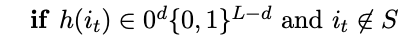
\includegraphics[width=0.4\linewidth]{img/image_2023-02-10-12-37-38.png}
            \caption{Treat notation here like a regexp; i.e. $ d  $ $ 0 $-s followed by $ L-d $ $ 1 $s or $ 0 $s}
        \end{figure}
\end{enumerate}

This algorithm attempts to maintain set $ S  $ such that it contains each element that appears with probability $ 2^{-d} $ and therefore $ E[|S|] $ is $ 2^{-d} $ of the elements that appear in the stream\mn{So $ \hat{F}_0 = 2^d |S| $ }
$ k $ is a constant that we get to pick -- the larger it is, the more space our algorithm uses (but the more accurate it becomes).




\begin{definition}
    Recall: \textbf{Variance}: a measure of how much a random variable $ X $ deviates from its expectation on average, i.e. the expectation of the difference between $ X $ and it's expectation.
    \begin{equation}
        \begin{split}
            Var(X) &=  E[(X - E[X])^2] \\
                   &= E[X^2] - E[X]^2  \\
        \end{split}
    \end{equation}

    An useful property of variance is the sum of independent random variables is equal to the sum of their variances

    \begin{equation}
        Var(\sum_{i=1}^{N} X_i ) = \sum_{i=1}^{N} Var(X_i)
    \end{equation}
\end{definition}

Another tool that will be useful for this analysis is \textit{Chebyshev's Inequality}


\begin{definition}
    \textbf{Chebyshev's Inequality} 

    \begin{equation}
        P(|X - E[X]| > t) < \frac{Var(X) }{t^2}
    \end{equation}


    \begin{proof}
        A proof of this inequality follows from Markov's inequality discussed in the previous lecture on locality sensitive hashing.

        Define $ Z = (X - E[X])^2 $. Since this implies $ Z \ge 0  $ and $ Var(X) = E[Z] $ by definition,

        \begin{equation}
        |X - E[X]| > t \Leftrightarrow X > t^2
        \end{equation}

        So we can just apply Markov's inequality to the above statement to give

        \begin{equation}
            P(|X - E[X]| > t) = P(Z > t^2) < \frac{Var(X) }{t^2}
        \end{equation}

        A nice property of Chebyshev's inequality is that it doesn't assume the random variable is non-negative and bounds the probability in both directions as well.
    \end{proof}
\end{definition}


\begin{theorem}
    If $ \tilde{F}_0  $ satisfies our prior assertion that $ F_0 \le \tilde{F}_0 \le  2 F_0 $, then $ \hat{F}_0 $ output by $ \proc{distinct-simple}(\sigma, \tilde{F}_0, k) $ satisfies 

    \begin{equation}
        (1-\frac{\sqrt{8} }{\sqrt{k} }) \le  \hat{F}_0 \le  (1+\frac{\sqrt{8} }{\sqrt{k} }) 
    \end{equation}

    With probability $ > \frac{1}{2} $ and uses $ O(k) $ memory.


\begin{proof}

    Define $ D $  to be the set of $ i \in [n] $ that appear in the stream. By definition, $ F_0 = |D| $.
    Define $ X_i $ as an indicator random variable, i.e. 

    \begin{equation}
        X_i = \begin{cases}
            1 & \text{ if $ i \in D $} \\
            0 & \text{otherwise}
        \end{cases}
    \end{equation}

    Then,

    \begin{equation}
        E[X_i] = P(i \in S) = 2^{-d}
    \end{equation}

    Since $ h(i) $ is uniformly random in $ \left\{ 0, 1 \right\} ^L $ and by construction $ 2^{L-d}  $ of $ 2^L $ strings have $ d $ leftmost bits set to $ 0 $.

    Then,

    \begin{equation}
        E[|S|] = E[\sum_{i \in D} X_i] = \sum_{i \in D} P(i \in S) = 2^{-d} F_0
    \end{equation}

    Since we chose $ d $ such that $ 2^{-d} \tilde{F}_0 \le  k $, we have

    \begin{equation}
        E[|S|] \le 2^{-d}F_0 \le  2^{-d} \tilde{F}_0 \le k
    \end{equation}

    \marginnote{It follows that the algorithm takes $ O(k) $ memory in expectation since $ S $ dominates the memory use}

    However this is not enough to show that $ \hat{F}_0 $ is close to $ F_0 $ even though it is easy to see that they are equal in expectation.
    To show this we can apply Chebyshev's inequality, i.e. if the variance of $ \hat{F}_0 $ is small it is likely to be close to its expectation.


    We know that 

    \begin{equation}
        Var(|S|) = \sum_{i \in D}^{} Var(X_i)
    \end{equation}

    and that

    \begin{equation}
        Var(X_i) = E[X_i^2] - E[X_i]^2 \le  E[X_i^2] = 2^{-d}
    \end{equation}

    So we get $ Var(|S|) \le 2^{-d} F_0 = E[|S|] $

    So, if we let $ \varepsilon = \frac{\sqrt{8}}{\sqrt{k}} $, then by Chebyshev we get

    \begin{equation}
        \begin{split}
            P(\hat{F}_0 - F_0) \ge \varepsilon F_0) &= P(|\hat{F}_0 - E[\hat{F}_0|] \ge  \varepsilon E[\hat{F}_0]) \\
                                                    &= P(|S| - E[|S|] \ge  \varepsilon E[|S|]) \\
                                                    &\le \frac{Var(|S|)}{\varepsilon^2 E[|S|^2]} \le  \frac{1}{\varepsilon^2 E[|S|]}
        \end{split}
    \end{equation}

    So if the expected size of $ S $ is not too small we have a large probability of getting an accurate estimate.

    Rearranging, our prior choice that $ 2^d \le  2 \tilde{F}_0 /k $, we get 

    \begin{equation}
        E[|S|] = 2^{-d} F_0 \ge  2^{-d-1} \tilde{F}_0 \ge  \frac{k}{4}
    \end{equation} 

    Plugging this bound for $ E[|S|] $ into the expression obtained by Chebyshev's inequality we get 

    \begin{equation}
        P( |\hat{F}_0 - F_0 | \ge  \varepsilon F_0) \le  \frac{4}{\varepsilon^2 k} = \frac{1}{2}
    \end{equation}
    
\end{proof}
    
\end{theorem}






\subsubsection{Adaptive Sampling}

A single-pass streaming algorithm for distinct counts which does not assume an estimate $ \tilde{F}_0 $.


\begin{codebox}
\Procname{$\proc{Distinct}(\sigma, k)$}
\li $ S = \emptyset, d = 0, L = \left\lceil \log_2 n  \right\rceil  $
\li Pick a hash function $ h: [n] \to  \left\{ 0, 1 \right\} ^L $
\li \For $ t \gets 1 \to m $ \Do
\li     \If $ h(i_t) \in 0^d \left\{ 0, 1 \right\} ^{L-d}  $ and $ i_t \notin S $ \Then
\li         $S = s \cup \left\{ i\_t \right\} $ \End
\li     \While $ |S| > k $ \Do
\li     $  d= d+1$
\li     $ T = \emptyset $
\li     \For $ j \in S  $
\li         \If $ h(j) \in 0^d \left\{ 0, 1 \right\} ^{L-d} $ \Then
\li             $ T = T \cup \left\{ j \right\} $ \End
\li     $ S = T $ \End \End \End
\li \Return $ \hat{F}_0 = 2^d \cdot  |S| $
\end{codebox}

\begin{blockquote}
    The idea behind this algorithm is to apply the concepts in $ \proc{Distinct-Simple} $ to set $ d $ and the sample rate adaptively while keeping the invariant of $|S| \le k$.
\end{blockquote}


\begin{theorem}
    Let $ 0 \le \varepsilon \le  \frac{1}{3}  $ and $ k \ge  \frac{16}{\varepsilon^2} $.\mn{In the lecture note we use $ k \ge  144 $ to get a bound with $ \varepsilon = \frac{4}{\sqrt{k}} $} Then, with probability at least $ \frac{1}{2} $ the estimate $ \hat{F_0} $ output by $ \proc{Distinct}(\sigma, k) $ satisfies

    \begin{equation}
        (1-\varepsilon) F_0 \le  \hat{F}_0 \le (1+\varepsilon) \cdot F_0
    \end{equation}
\end{theorem}

\begin{proof}
    Let $ D = \left\{ i : f_i > 0 \right\}  $ be the distinct elements that appear in $ \sigma $, and  $ S_l = \left\{ i \in D : h(i) \in 0^l \left\{ 0,1 \right\} ^{L-l} \right\}  $ be the elements in $ \sigma $ whose hash value starts with $ l $ zeros.
    By this definition $ |D| = F_0 $.

    \begin{equation}
    E[|S_l|] = 2^{-l} |D| = 2^{-l} F_0
    \end{equation}

    \begin{equation}
        Var[|S_l|] = 2^{-l} (1-s^{-l}) \le  E[|S_l|]  = 2^{-l} F_0
    \end{equation}
    

    At the end of $ \sigma $, $ d = min \left\{  l: |s_l| \le  k \right\} $. \mn{All of these variables here are random.}
    Can think of the algorithm as keeping $ s_0 $ at first, and then if there's too much in $ s_0 $ it will move on to $ s_1 $ and so forth.
    The output of the algorithm, $ \hat{F}_0 $ is given by $ 2^d |S_d| $. So this algorithm searches for the first $ l $ such that $ |S_l| \le  k$.
    Note that the expected sizes of $ S_l $ halve with each increment in $ l $.


    For correctness we need

   \begin{equation}
       a == \left\lfloor \log_2 ((1-\varepsilon) F_0 / k )  \right\rfloor
       b == \left\lceil  \log_2 ((1+\varepsilon) F_0 / k )  \right\rceil 
   \end{equation}

   Chosen such that $  a \le  d \le  B$

   \begin{equation}
       \frac{(1-\varepsilon) F_0}{2k} \le  2^a \le  \frac{(1-\varepsilon) F_0}{k}
   \end{equation}

   This implies that 

   \begin{equation}
       (1+\varepsilon E[|S_a|]) = (1+\varepsilon) 2^{-a} F_0 \ge  k
   \end{equation}
   

   \begin{equation}
       \frac{(1+\varepsilon) F_0}{k} \le  2^b \le  \frac{2(1+\varepsilon) F_0}{k}
   \end{equation}

   This implies that

   \begin{equation}
       (1+\varepsilon) E|S_b| \le  k
   \end{equation}


   We will now show that the following probabilities $ \ge  \frac{5}{6}  $ which is $ \ge \frac{1}{2} $, which implies that the probability of all 3 is at least $ \frac{1}{2} $.


   \begin{equation}
       (1-\varepsilon) F_0 < 2^a |S_a| \le  (1+\varepsilon)F_0 \ge  \frac{5}{6}
   \end{equation}

   For this one:


   \begin{equation}
       \begin{split}
           \Rightarrow |S_a| &> (1-\varepsilon) 2^{-a} \qquad F_0 \ge  k  \\
            |S_a| & > k \Rightarrow a < d  \\
       \end{split}
   \end{equation}

   \begin{equation}
       |S_b| \le  k \Rightarrow d \le  b
   \end{equation}
   
   

   
   \begin{equation}
       (1-\varepsilon) F_0 < 2^{b+1} |S_{b-1}| \le  (1+\varepsilon)F_0 \ge  \frac{5}{6}
   \end{equation}


   \begin{equation}
       (1-\varepsilon) F_0 < 2^b |S_b| \le  (1+\varepsilon)F_0 \ge  \frac{5}{6}
   \end{equation}


   Note: if $ \varepsilon $ small enough and after some calculations we can show that 

   \begin{equation}
       B \le  a + 2
   \end{equation}
   
   \begin{equation}
       (1-\varepsilon)|S_a| = (1-\varepsilon) 2^{-a} F_0 \ge k
   \end{equation}

\end{proof}





\subsection{Linear Programming}


A linear programming is an optimization problem defined by linear inequalities and equalities. The following form will be used in this class:


\begin{definition}
    Linear program:

    \begin{equation}
        max \text{  }c^T x \text{ s.t. } Ax \le  b \qquad x \ge 0
    \end{equation}

    Where $ A  $ is a $ m\times  n $ matrix ($ m $ constraints, $ n $ variables), $ b $ is a $ m \times  1$ column vector. $ c $ is a $ n \times  1 $ column vector, and $ x $ is a $ n \times  1 $ objective column vector. The inequalities are such that the inequality should hold for all elements of the above matrix expression at the same time.
    The set of $ x $ that satisfy the constraints is called the feasible set, and the LP is \textit{infeasible} if the feasible set is empty.
    
\end{definition}

For example,

\begin{equation}
    \begin{split}
        min x_1 + x_2 + x_3 & s.t. \\
         x_1 + x_2 &= 1  \\
         x_2 + x_3&\ge  1 \\
         x_1 + x_3 &\ge  1 \\
         x_1, x_2, x_3 &\ge  0
    \end{split}
\end{equation}

Which corresponds to the following matricies

\begin{equation}
    \begin{split}
        A = \begin{bmatrix}
            1 & 1 & 0 \\
            0 & 1 & 1 \\
            1 & 0 & 1
        \end{bmatrix} \qquad b = \begin{bmatrix}
            1 \\
            1 \\
            1
        \end{bmatrix} \qquad c = \begin{bmatrix}
            1 \\
            1 \\
            1
        \end{bmatrix}
    \end{split}
    \label{eq:lp1}
\end{equation}

Geometrically we may understand LPs as some sort of $ n $-dimensional polyhedron comprised of the intersection of the halfspaces defined by the hyperplanes each inequality represents.
In more simple terms: each inequality defines a supporting hyperplane $ \left\{ x \in \mathbb{R}^n : a^Tx = b \right\}  $ One \textit{halfside}, $ \left\{ x \in \mathbb{R}^n: a^T x \le  b \right\}  $ of the hyperplane gives admissible solutions to the inequality.
The polyhedron that contains all of the solutions to the inequality is then given by the intersection of all the hyperplanes in the set.
A polyhedron $ P $ is \textit{unbounded} when there exists a point $ x $ such that $ x \in P $ and a direction $ v $ for which for every $ t \ge  0 $, $ x + tv \in P $. A bounded polyhedron, i.e. not unbounded is a \textit{polytope}.

\begin{definition}
Formally a \textbf{face} of a polyhedron is a set of the type 

\begin{equation}
    F = \left\{  x : Ax \le  b \right\}  \cap \left\{  x : a_ix = b_i \forall i \in S \right\}
\end{equation}

Where $ a_i $ is the $ i $th row of $ A $ and $ S $ is some subset of the rows of $ A $. 

A {j-face} is a face where the rank of the sub-matrix $ A_f $ of $ A $ for that face is $ n-j $. 

\begin{figure}[H]
    \centering
    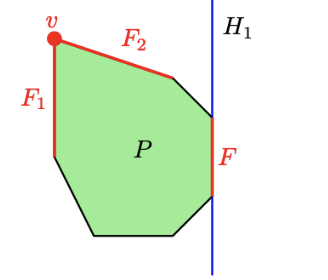
\includegraphics[width=0.8\linewidth]{img/image_2023-03-08-16-28-53.png}
    \caption{In this example the triangle $ \left\{ (1,0,0), (0,1,0), (0,0,1) \right\}  $ is a facet (2-face); $ F = P \cup \left\{ x_1 + x_2 + x_3 = 1 \right\}  $. The edge $ F_1 $ or $ F_2 $ is a 1-face, and the vertex $  v $ is a 0-face}
\end{figure}
 
    
\end{definition}



\begin{definition}
    A \textbf{Vertex} of a polytope $ P = \left\{ x \in \mathbb{R}^n : Ax < b \right\}  $  is a point in $ P $ we  can get by setting $ n $ linearly independent constraints to equality

    \begin{equation}
        \begin{split}
            x_1 + x_2 &\ge 10 \implies x_1 + x_2 = 10  \\
             x_2 + x_3 &\le 15 \implies x_2 + x_3 = 15 \\
        \end{split}
    \end{equation}

\end{definition}

\begin{theorem}
    For any polytope $ P $ with verticies $ v_1 \ldots v_N $, any $ x \in P $ can be witten as $ x = \lambda_1 v_1 + \ldots + \lambda_N v_N $, where

    \begin{equation}
        \sum_{i=1}^N \lambda_i = 1
    \end{equation}

    And

    \begin{equation}
        \lambda_i \ge 0
    \end{equation}

\end{theorem}


\begin{theorem}
    Vertices $ v \in P $ are optimal solutions to the LP, i.e. $ c^Tx$  is minimized or maximized.
\end{theorem}





\begin{definition}
    \textbf{Convexity}: A set $ S \in \mathbb{R}^n $ is convex if for any two points $ x, y $ in $ S $ the line segment between $ x $ and $ y $ is contained in $ S $.
\end{definition}

\begin{definition}
    \textbf{Convex Hull}: $ v_1, \ldots, v_n \in \mathbb{R}^n $ is the smallest convex set of $ S \in \mathbb{R}^n  $ containing $ v_1 \ldots, v_N $.
    This can be imagined as a \textit{shrink-wrap} of the points.
    \begin{figure}[H]
        \centering
        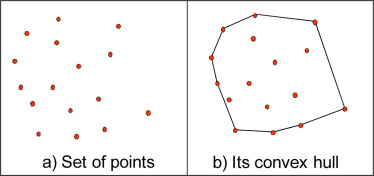
\includegraphics[width=0.8\linewidth]{img/image_2023-03-08-12-25-32.png}
    \end{figure}

    Algebraically this can be written as

    \begin{equation}
        \proc{conv-hull}(\left\{ v_1 \ldots, v_N\right\} ) =
        \left\{ \lambda_1 v_1 + \ldots, h_N v_N : \lambda_1 \ldots, \lambda_N \ge 0, \lambda_1 + \ldots, + \lambda_N = 1 \right\} 
    \end{equation}

    Many proofs involving convex hulls may be partially resolved with the fact that the convex hull of two points is the line between them, and a little bit of induction.
\end{definition}

\subsubsection{LP Examples}

\begin{blockquote}
    In order to use linear programming we must need to know how to frame questions as LP questions.
\end{blockquote}

\begin{example}
    Menu planning

    Given the following list of prices \& nutritional values for a set of foods, find the minimum additional price for dish to meet nutritional requirements?
    \begin{figure}[H]
        \centering
        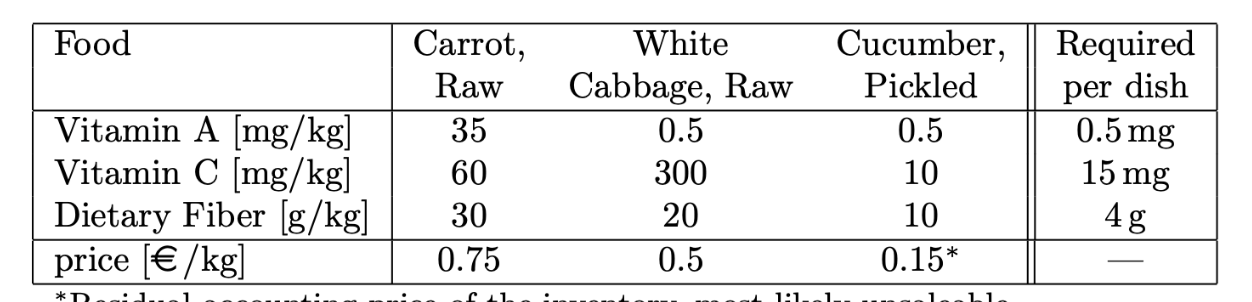
\includegraphics[width=0.8\linewidth]{img/image_2023-03-08-16-37-59.png}
    \end{figure}


    \begin{figure}[H]
        \centering
        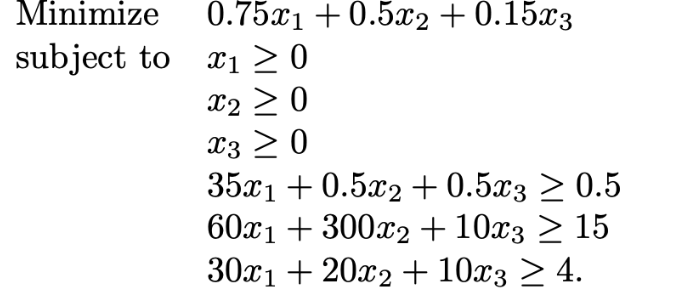
\includegraphics[width=0.8\linewidth]{img/image_2023-03-08-16-38-07.png}
    \end{figure}

    The minimization is simply the price multiplied by the amount. The constraints can be described as follows:

    \begin{itemize}
        \item There should be non-zero carrots, white cabbage, and pickles
        \item The sum of vitamin A across the dish should be at least 0.5mg
        \item And so forth...
    \end{itemize}

\end{example}

\begin{example}
    Network flow
    \begin{figure}[H]
        \centering
        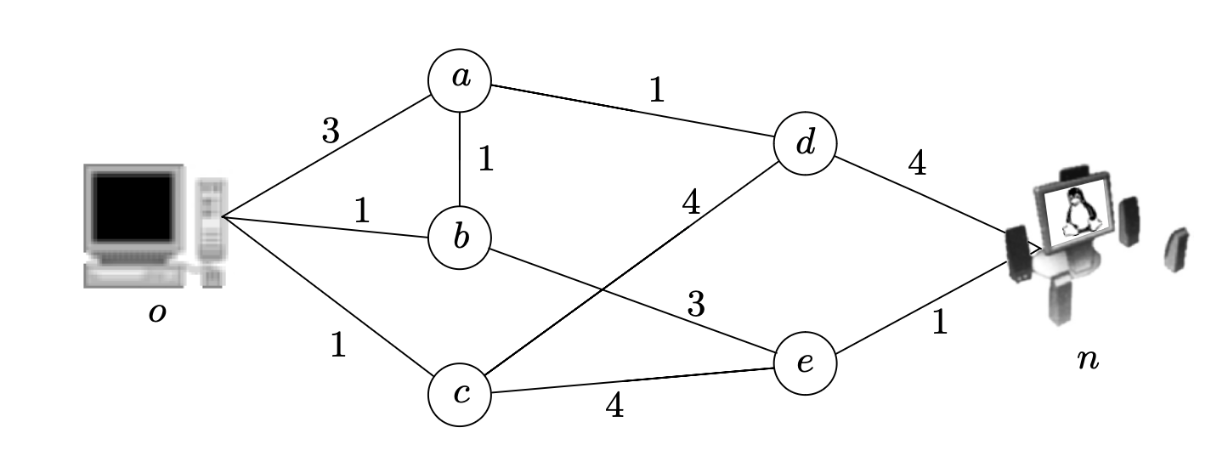
\includegraphics[width=0.8\linewidth]{img/image_2023-03-08-16-40-21.png}
    \end{figure}

    What is the maximum transfer rate from the old computer $ o $ to the new computer $ n $?

    Let's introduce a variable $ x_{ab} $ which specifies the rate at which data is transferred from $ a  $ to $ b $ for each link in the network. In this graph we have 10 such variables.

    The linear program is then as follows

    \begin{figure}[H]
        \centering
        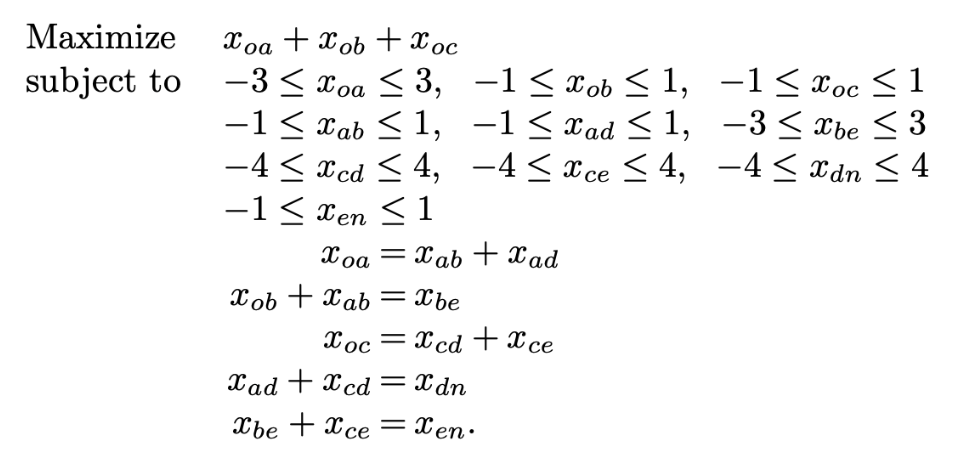
\includegraphics[width=0.8\linewidth]{img/image_2023-03-08-16-42-20.png}
    \end{figure}

    Our goal is to maximize the flow out of computer $ o $ under the assumption that, since the data is neither stored or lost, it must be received by $ n $ at the same rate.
    The next constraints restrict the transfer rates along each of the individual links, i.e. $ x_{cd} $ can transmit at a rate of up to $ 4  $ forwards or backwards ($ -4 \le  x_{cd \le  4}$).
    The relations between the nodes are then captured in the last few equality constraints and effectively say that whatever leaves each node must leave it immediately \mn{$ x_{oa} = x_{ab } + x_{ad}$; flow from $ o \to  a $ must leave through $ a $ to either $ b , d $}.


\end{example}

Consider the following problem: given a projected mostly ice cream sales for the next year, how can produce a production schedule with the minimum cost?

\begin{example}
    \begin{figure}[H]
        \centering
        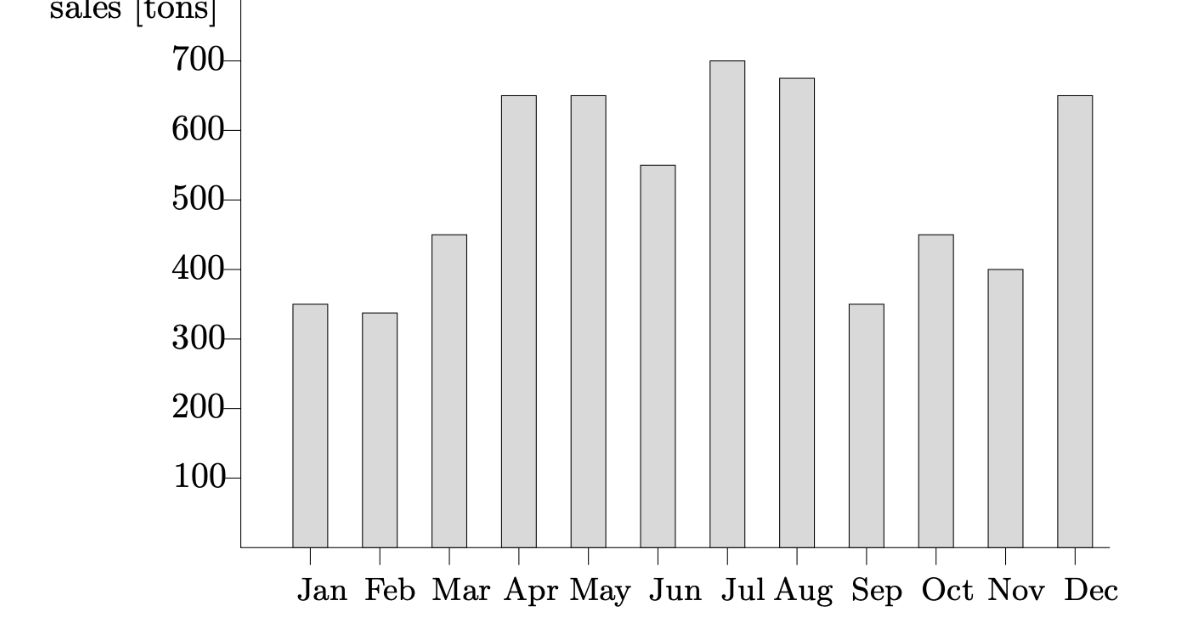
\includegraphics[width=0.8\linewidth]{img/image_2023-03-08-16-47-17.png}
    \end{figure}
\end{example}

A simple solution might be JIT\mn{just-in-time (heh)} production -- but this can be expensive due to temp workers and machine adjustments, etc. 
It may be better to spread out production and to build up stock.


Let's formalize this problem as follows:

\begin{itemize}
    \item Demand in month $ i $ is $ d_i $
    \item $ x_i $ is the production in month $ i $
    \item $ s_i $ is the total surplus in store at end of month $ i $
    \item To meet demand in month $ i $ we may use the production in month $ i $ and the surplus from $ i-1 $; $ x_i + s_{i-1} \ge  d_i $
    \item And the surplus after month $ i $ is $ x_i + s_{i-1} - s_i = d_i $
    \item Assume initial surplus is $ s_0 = 0 $, and we want $ s_{12} = 0 $
\end{itemize}

Let's take the cost of changing production by 1 ton between two months to be $ 50 $ and the storage cost for 1 ton of ice cream is $ 20 $

Total cost:

\begin{equation}
    50 \sum_{i = 1}^{12} |x_i - x_{i-1}| + 20 \sum_{i = 1}^{12} s_i
\end{equation}

This cost function is unfortunately not linear, but we can use the following trick to make it linear: since the change in production is either an increase or decrease, we may introduce $ y_i \ge  0 $ for the increase and $ z_i \ge 0 $ for the decrease to get

\begin{equation}
    x_i - x_{i-1} = y_i - y_z \qquad \text{and} \qquad |x_i - x_{i-1}| = y_i + z_i
\end{equation}

\begin{figure}[H]
    \centering
    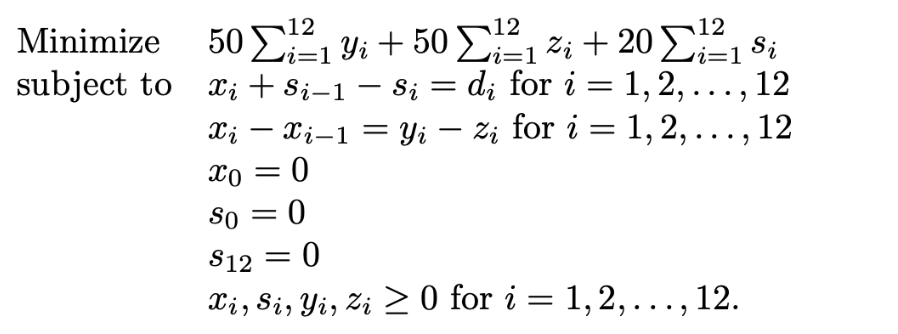
\includegraphics[width=0.8\linewidth]{img/image_2023-03-08-16-54-39.png}
    \caption{The linear program that follows}
\end{figure}










\subsubsection{Duality}

How can I convince you that the solution to a linear program is optimal?


\begin{equation}
    \begin{split}
        \max &  x_1 \\
        \text{given} &\\
        x_1 + x_2 + x_3 &\le  1 \\
        x_1 \cdot  x_2 \cdot  x_3 \ge  0 \\
    \end{split}
\end{equation}

We know that the optimal value of this LP is $ x_1 = 1, x_2 = 0, x_3 = 0 $.

Or, to solve the example given at the beginning of this section (equation \ref{eq:lp1}), we have the solution\marginnote{Note symmetry in solution!} $ x_1 = x_2 = x_3 = \frac{1}{2} \implies \text{value } \le  \frac{3}{2} $.

If we were to multiply each inequality by half and add them up, we get

\begin{equation}
    x_1 + x_2 + x_3 \ge  \frac{3}{2}
\end{equation}

So here we were able to put a lower bound on the optimal value of the LP, but we don't know abut the upper bound. We can do this by using duality.
Before we do that, here's the above logic formalized:

Given the $ LP $ in general form

\begin{equation}
    \max c^T x \text{ s.t. } Ax \le  b \qquad x \ge 0
\end{equation}

We may apply the technique of dropping values and multiplying the inequalities used above.

Let's define $ y \ge 0 $ as the dual variables which are applied onto the inequality as follows:

\begin{equation}
    y(Ax \le  b)
\end{equation}

\begin{blockquote}
    Only multiply by non-negative constants to avoid messing up the inequalities
\end{blockquote}

Then,

\begin{equation}
    yAx \le  yb
\end{equation}

If every row of $ yA $ is greater than equal to $ c_i $, then the objective value is upper-bounded by $ yb $!

And as it turns out this is just yet another linear program for minimization over choices of $ y $ that we can solve with our existing LP techniques.
\marginnote{
    if $ \max c^Tx \text{ where }Ax \le  b, x\ge 0$ is the original LP, we call it the \textbf{primal} LP, and $ min b^Ty \text{ where } A^Ty\ge c, y \ge 0   $ is the \textbf{dual} LP. Refer to handout for more primal-dual pairs.}


\begin{theorem}
    Weak duality: Let $ x $ satisfy the primal LP, and let $ y $ satisfy the dual constraints. Then, $ c^Tx \le  b^Ty $.
\end{theorem}

The proof follows from observing that the primal LP is a maximization problem and the dual is a minimization problem. Then a solution to the maximization problem is lesser than it's dual minimization problem. More formally,

\begin{proof}
    Observe that
\begin{equation}
    u, w, v \in \mathbb{R}^n, u \ge  v, w \ge 0 \text{ then  } u^Tw \ge v^Tw
\end{equation}

Then, since we have $ c \le  A^T y $ and $ x \ge 0 $, we have $ c^Tx \le  y^T Ax $\marginnote{Think of the connection between the dual linear programs; $ b $ and $ c $ appear in both the primal and dual problems}. Likewise, we have $ y^TAx \le  y^T b $. So,

\begin{equation}
    c^Tx \le  y^T Ax \le  y^T b \implies c^Tx \le  b^Ty
\end{equation}
    
\end{proof}



\begin{theorem}
    If both primal and dual LPs are feasible, then their optimal values are equal.
\end{theorem}

The proof of this theorem lies on Farkas' Lemma.

\begin{lemma}
    \textbf{Farkas's Lemma}: For any $ m \times  n $ matrix $ A $ and any $ m \times 1 $ vector $ b $, exactly one of the following two statements is true

    \begin{enumerate}
        \item There exists a $ x \in \mathbb{R}^n, x \ge  0  $ such that $ Ax = b $
        \item There exists a $ y \in R^m $ such that $ A^Ty \le  0 $ and $ b^Ty > 0 $ 
    \end{enumerate}

\end{lemma}



\begin{figure}[H]
    \centering
    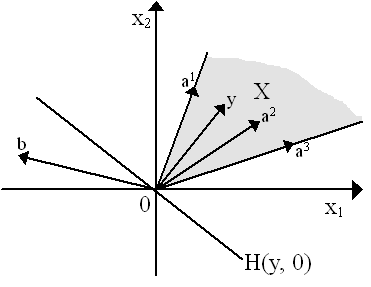
\includegraphics[width=0.8\linewidth]{img/image_2023-03-29-12-40-27.png}
\end{figure}

\begin{blockquote}
We can think of Farkas's Lemma as a conclusion made about the geometry of the problem.
We define a hypercone $ C$ with the first constraint, $C = \left\{ Ax: x \ge 0 \right\} $.
If the first statement does not hold, then we have $ b \notin C $.
Now what we aim to show is that, if $ b \notin C $, then there exists a hyperplane $ H $ through the origin that splits the space such that the hypercone lies entirely on one side of $ H $ and $ b $ is on the other side.

\begin{figure}[H]
    \centering
    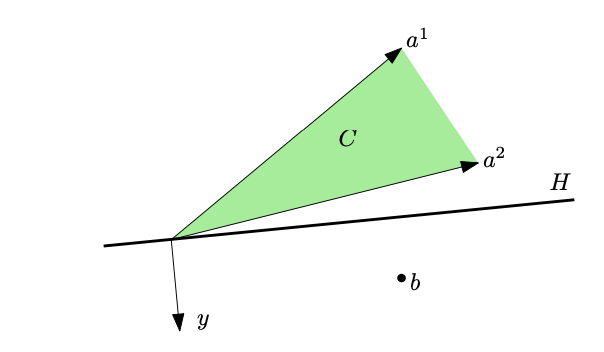
\includegraphics[width=0.8\linewidth]{img/image_2023-04-03-15-54-43.png}
\end{figure}
    
\end{blockquote}

Using Farkas's Lemma, we can prove the theorem.
Since we assume that the primal and dual are feasible, then their values $ v_p, v_d $ are finite and achieved. 
Since the optimal value of the dual LP is $ v_d $, there does not exist any $ y \in \mathbb{R}^m$ such that $ y \ge 0  $, $ A^ty \ge c $, and $ y^tb < v_d$. 
This implies that the intersection of the hyperplane and $ P $  is non-empty and $ v_p \ge  v_d $. However, by weak duality $ v_p \le d $. Therefore, $ v_p = v_d $.

\begin{figure}[H]
    \centering
    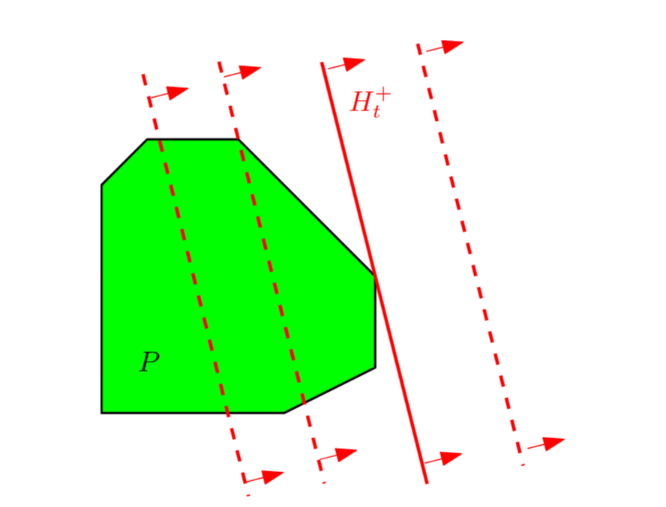
\includegraphics[width=0.8\linewidth]{img/image_2023-04-06-02-03-46.png}
\end{figure}


\marginnote{Also, if we take the dual of a LP twice we get the original LP back}


\begin{theorem}
    \textbf{Complementary Slackness}

    Let $ x $ be a feasible solution to the primal LP, and let $ y $ be a feasible solution to the dual LP. Then $ x, y $ are optimal if and only if:

    \begin{equation}
        \forall i \in \left\{  1 \ldots,  m \right\} : (b_i - (Ax)_i)y_i = 0
    \end{equation}

    \begin{equation}
        \forall j \in \left\{  1 \ldots,  n \right\} : ((A^Ty)_j - c_j)x_j = 0
    \end{equation}

    \begin{proof}
        $ x $ and $ y $ are optimal $ \iff $ $ c^Tx = b^Ty = v $, so

        \begin{equation}
            y^T Ax \le  y^T b = v = c^Tx \ge  y^T Ax \Rightarrow y^T Ax = c^Tx = y^T b
        \end{equation}


    \end{proof}
    
    In other words, a primal feasible solution $ x $ and dual feasible solution $ y $ are optimal if and only if whenever a dual variable $ y_i $ is positive, the corresponding primal constraint is tight ($ (Ax)_i = b_i$). Similarly, whenever a primal constraint is slack ($ (Ax)_i < b_i $), then the corresponding dual variable is 0. The same applies in the opposite direction; whenever a primal variable $ x_j $ is positive, the corresponding dual constraint is tight ($ (A^ty)_j = c_j $), and if the dual constraint is slack ($ (A^ty > c_j) $) then the dual variable is $ 0 $. In more concise terms at most one of the constraints in each pair is slack.

    
    



\end{theorem}


\subsection{Bipartite Matching}

A bipartite graph is a graph whose vertices can be partitioned into two disjoint sets $ A, B $ such that every edge connects a vertex in $ A $ to a vertex in $ B $. A matching $ M $ is a subset of edges such that each vertex of $ V $ is incident to at most one edge of $ M $. An exposed vertex $ v $ has no edge of $ M $ incident to it. A perfect matching has no exposed vertex

\subsubsection{Maximum Cardinality Matching}
The goal of the Maximum Cardinality Matching problem is to find a matching of maximum size.
There exists a duality between the size of the upper bound of the maximum cardinality matching and the lower minimum size of a vertex cover.
By definition, a vertex cover $ C $ is a set such that all edges are incident to at least one vertex in $ C $. 
Weak duality (the maximum size of a matching is at most the minimum size of a vertex cover) follows because for any matching $ M $, $ C $ must contain at least one of the endpoints of each edge in $ M $.

\begin{theorem}
    Strong duality between the maximum size of a matching and the minimum size of a vertex cover holds for bipartite graphs.
\end{theorem}

\begin{definition}
    \textbf{Alternating path}: An alternating path in $ M $ is one that alternates between edges in $ M $ and $ E-M $
\end{definition}

\begin{definition}
    \textbf{Augmenting Path}: An augmenting path with respect to $ M $ is an alternating path that starts and ends at exposed vertices.
\end{definition}

Note that an augmenting path w.r.t. $ M $ contains $ k $ edges of $ M $ and $ k+1 $ edges not in M. And the endpoints must be on different sides of the bipartition, so if we get

\begin{equation}
    M' = M \Delta P \equiv (M-P) \cup (P-M)
\end{equation}

where $ P $ is the augmenting path we get a new matching $ M' $ that is one edge larger than $ M $, i.e. $ |M'| = k + 1 $.

\begin{theorem}
    A matching $ M $ is maximum if and only if there is no augmenting path w.r.t. $ M $.
    The proof is simple via a proof by contradiction from the definition of an augmenting path.
\end{theorem}


An algorithm for finding a maximum matching is to start with an empty matching and repeatedly find an augmenting path and add it to the matching. 
We know that it will terminate by the theorem above, and specifically, it will terminate after $ O(\mu) $ augmentations, where $ \mu $ is the size of the maximum matching. \marginnote{We know $ \mu \le  \frac{n}{2}$ given a bipartite graph}
This sounds great, but how can we find an augmenting path? Construct directed graph $ D $ which is a copy of $ G $ but with edges directed such that there is a path from $ A \to B $ if it does not belong to $ M $ and $ B \to A $ otherwise.
There exists an augmenting path in $ G $ with respect to $ M $ $ \iff $ there exists a directed path in $ D $ between exposed vertices in $ A $ and $ B $. DFS can be used on this graph to give an $ O(m) $ algorithm to finding an augmenting path in $ G $, leading to an $ O(nm) $ algorithm for maximum cardinality matching which can be cut down to $ O(m \sqrt{n})$ by augmenting among several paths at the same time.

When the algorithm terminates, $ C* = (A-L) \cup (B \cap L) $ is a vertex cover, and $ |C*| = |M*|$

\begin{proof}
    A proof by contradiction can be used to show that it is a vertex cover.

    Suppose $ C* $ is not a vertex cover. Then $ \exists e = (a,b)  $ with $ a \in A\cap L $ and $ b \in B - L $, i.e. cannot belong to the matching. This means that $ e $ is in $ E - M $ and was directed (in $ D $) from $  A \to B $.
    This implies that $ b $ can be reached from an exposed vertex in $ A $  via a directed path in $ D $ through $ e $\mn{Since it is the only such edge} which contradicts that $ b \in B-L $.


    The second part of the proof, that every vertex in $ C $ covers exactly one edge in $ M $ follows from

    \begin{itemize}
        \item No vertex in $ A-L $ and $ B \cap L $ is exposed, by definition or by the fact that the algorithm terminates.
        \item There is no edge of the matching between $ A-L $ and $ B \cap L $, otherwise $ a $ would be in $ L $
    \end{itemize}

    This implies that every vertex in $ C* $ is matched and the corresponding edges are distinct -- so $ |C*| \le  |M*| $. The opposite direction holds by weak duality, so $ |C*| = |M*| $.

\end{proof}


\subsubsection{Minimum Weight Perfect Matching}

\begin{blockquote}
    There are $ n $ jobs and $ n $ workers. Each job $ i $ requires a worker $ j $ to complete it. Each worker $ j $ has a cost $ c_j $ to work on a job. Find a task assignment of minimum cost.
\end{blockquote}

\begin{itemize}
    \item Assume $ G $ has a perfect matching $ M $, $ |M| = \frac{n}{2} $. Also assume that it is a complete bipartite graph, i.e. $ \exists e=(a,b) \forall a \in A, b \in B $
\end{itemize}


The minimum weight perfect matching problem may be formulated as follows:

\begin{equation}
    \begin{split}
        \min \sum_{i, j} c_{ij} x_{ij} & \text{ subject to}  \\
         \sum_j x_{ij} = 1 &\qquad i \in A  \\
         \sum_i x_{ij} = 1 &\qquad j \in B  \\
         x_{ij} \ge  0 &\qquad i \in A, j \in B \\
                       & x_{ij} \text{is an integer}
    \end{split}
\end{equation}

\marginnote{Convince yourself that any solution to this problem corresponds to a matching}

This is an \textit{integer problem}, which is a special case of the \textit{linear program} problem where the solutions must be integers.
A \textit{relaxed} problem, the linear program $ P $ is defined similarly to the integer program, but without the constraint that $ x_{ij} $ is an integer
\begin{figure}[H]
    \centering
    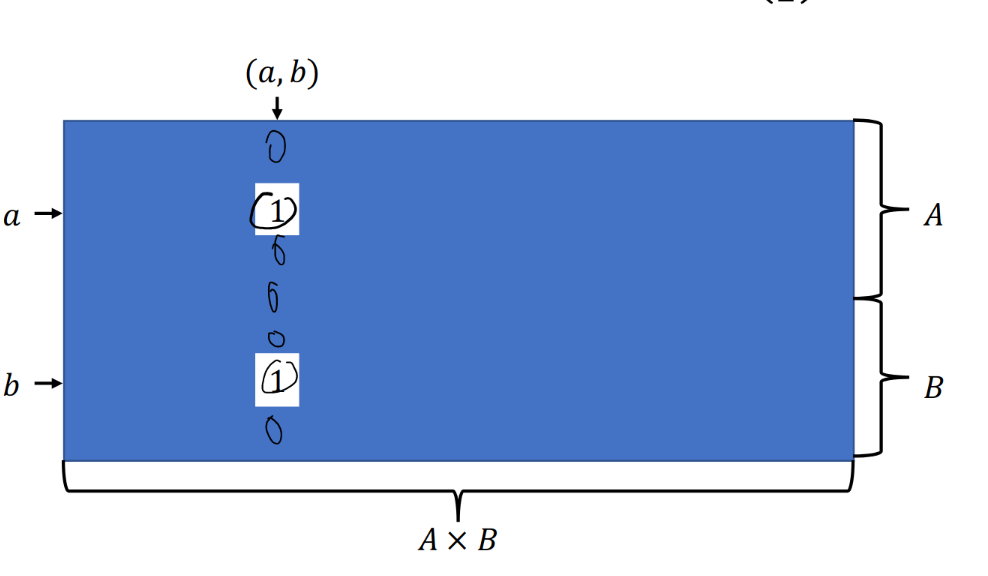
\includegraphics[width=0.8\linewidth]{img/image_2023-04-06-03-54-44.png}
\end{figure}
\begin{equation}
    \begin{split}
        \min \sum_{i, j} c_{ij} x_{ij} & \text{ subject to}  \\
         \sum_j x_{ij} = 1 &\qquad i \in A  \\
         \sum_i x_{ij} = 1 &\qquad j \in B  \\
         x_{ij} \ge  0 &\qquad i \in A, j \in B
    \end{split}
\end{equation}

We can see that if a linear program relaxation has an integral solution then it must be an optimum solution to the integer program.
In the special case of the perfect matching problem the constraint matrix has a special form and the following theorem holds


\begin{theorem}
    Any extreme point of the relaxed problem $ P $ is a $ 0-1 $ vector and is the incidence vector of a perfect matching
\end{theorem}

The \textbf{Hungarian Algorithm} solves this problem in $ O(n^3) $ time.


\begin{codebox}
\Procname{$\proc{hungarian}(G)$}
\li $  y = 0, M = \emptyset$
\li \While $ M $ is not perfect \Do 
\li     \If $ \exists $ augmenting path $ P  \in  G_y = (A \cup B, E_y) $ \Then 
\li         $ M = M \Delta P $
\li     \Else
\li         modify $ y $ while maintaining $ M \subseteq E_y $ \End \End
\end{codebox}

\begin{blockquote}
    Assume cost $ c_{ab} $ is non-negative. For any matching $ M $ we may formulate the dual problem: $ \forall a \in A, b \in B $, $ y_a + y_b \le  c_{ab} $. Then, to minimize the cost, we aim to maximize the dual linear program corresponding to $ y_a + y_b $. Also, define $ E_y $ to be the set of tight edges corresponding to some solution $ y $, i.e. $ E_y = \left\{ (a,b): y_a + y_b = c_{ab} \right\}  $

\end{blockquote}

\begin{itemize}
    \item Start with some dual feasible solution, i.e. $ y =0  $. 
    \item Repeatedly augment $ M $ until it is perfect. At every time step if we can't augment $ M $ using tight edges then we modify $ y $ until we can.
    \item Our goal is to find a perfect matching $ M $ while also satisfying the invariant $ M \subseteq E_y $    \item By maintaining the invariant we have, by complementary slackness, that $ M $ is a min cost perfect matching\mn{$ M $ is a perfect matching and $ M \subseteq E_y $ is comprised of tight edges, so the slack bounds on $ y $ are OK and in fact still lead to $ M $ being an optimal min cost perfect matching}
\end{itemize}

We had previously handwoven how to modify $ y $. 

\begin{itemize}
    \item Let $ G_{y, M} $ be a directed graph with edges in $ M $ from $ B \to A $ and edges not in $ M $ from $ A \to B $. By extension $ G_{y, M} $ is also a graph of tight edges
    \item Let $ U $ be the set of exposed vertices and $ L $ be vertices reachable in $ G_{y, M} $ from $ U \cap A$. 
        \begin{figure}[H]
            \centering
            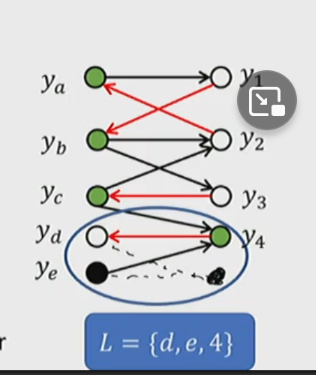
\includegraphics[width=0.8\linewidth]{img/image_2023-04-06-04-28-29.png}
            \caption{In other terms: $ L $ is the set of vertices reachable from the left side of the bipartite graph through the directed graph we built, from an exposed (unmatched) vertex}
        \end{figure}

    \item Assume no augmenting path exists. Then $ U \cap L \cap B  = \emptyset $. 
    \item By K\"oning's theorem, no edges of $ G_y $ are between $ A \cap L $ and $  B - L $
    \item Define $ \delta = \min \left\{ c_{a,b} - y_a - y_b: a \in A \cap L, b \in B - L \right\} > 0  $. In other words take a subset of the vertices and add/subtract a small value to/from the vertices in the subset, in our case the largest value such that $ y $ is still feasible, since adding smallest $ c_{ab} - y_a - y_b $ to $ y_a $ or subtracting it from $ y_b $ still permits the inequality $ y_a + y_b <= c_{ab} $ to hold.
        Apply modifications

        \begin{itemize}
            \item $ y_a \leftarrow y_a + \delta $ for $ a \in A \cap L $
            \item $ y_b \leftarrow y_b - \delta $ for $ b \in B - L $
        \end{itemize}
\end{itemize}

By definition after the modification with $ \delta $ $ y $ is still feasible. Also, $ M \subseteq E_y $ after modification still since if $ (a,b) \in M, b \in B \cap L   $ , then $ a \in A \cap L $.
All reachable vertices are still reachable in the new $ G_{y, M}$, and $ b $ is now newly reachable from $ a $.

On termination we have an incidence vector of a perfect matching and a dual feasible solution. By complementary slackness they must therefore be optimal.
Since we picked the perfect matching from tight edges we have also proved an integral solution to the linear program relaxation, and therefore an optimal solution to the integer program.


The presented approach is $ O(n^4) $: Each $ \le \frac{n}{2} $ modifications to $ y $, $ M  $ grows by 1 edge\mn{Each modification to $ y $ a new vertex in $ B $ enters $ L $, but only after $ \frac{n}{2} $ does an exposed vertex enter}. Total number of iterations is $ O(n^2) $, each of which are $ O(n^2) $. Better data structures can improve this to $ O(n^3) $





\subsection{Rounding \& Approximation Algorithms}

Many natural and important optimization problems are NP-hard. So what do we do? 

\begin{enumerate}
    \item Approximation: output an approximately optimal solution in worst-case polynomial time
    \item Algorithms that are efficient on special classes of the problem, i.e. Max Cut problem in planar graphs.
    \item Algorithms that are exponential in some parameter, i.e. $ 2^{O(k)} poly(n) $ and then hope that the parameter is small.
\end{enumerate}


\subsubsection{Min Weighted Vertex Cover}
One such problem that we may be interested in is the generalized vertex cover problem, which is NP-hard for general graphs. However, we may arrive at a Factor 2 approximation\mn{Can find a cover $ C $ in polynomial time such that $ w(C) \le  2 \cdot w(OPT)$ where $ OPT $ is the optimal solution} via formulations as an integer program, relaxing to an LP, and then rounding the possibly optimal LP solution to a $ \left\{ 0, 1 \right\}  $ IP solution (or something close to it).
In this section we will consider a generalization of the vertex cover problem, where we are given a graph $ G = (V, E) $ and vertex weights $ w \in R^V $ and we want to find a min-weight vertex cover (not just a vertex cover of min size).
\begin{figure}[H]
    \centering
    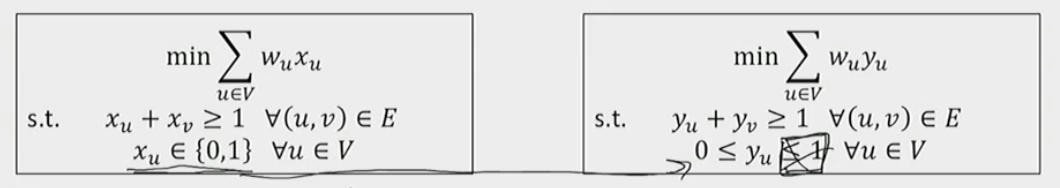
\includegraphics[width=0.8\linewidth]{img/image_2023-04-06-13-36-55.png}
    \caption{The IP is described by the constraint where $ x_u = 1 $ if $ u $ is in $ C $. The relaxation is the same but with the variables names changed and the integer constraint dropped. Also we can remove the constraint that $ y_u \le 1 $ if we want but in any case we are minimizing on $ y_u $ and we are rounding off to $ \left\{ 0, 1 \right\}  $ anyways}
\end{figure}


\subsubsection{Deterministic Rounding}
Our goal is to show that 

\begin{equation} 
    LP(G, w) \le OPT(G, w) \le 2 \cdot  LP(G, w)
\end{equation}

\begin{blockquote}
    Deterministic rounding: round to $ 1 $ if $ \ge \frac{1}{2} $ and $ 0 $ otherwise.
\end{blockquote}

Let $ y $ be an optimal solution and define the set $ C $ of vertex cover vertices from the LP

\begin{equation}
    C = \left\{  u \in V : y_u \ge  \frac{1}{2} \right\} 
\end{equation}


For this scenario $ x_u = 1 $ in the integer program implies $ u \in C $ and therefore $ y_u \ge \frac{1}{2} $ in the LP. Conversely if $ x_u = 0 $ in the IP then $ y_u < \frac{1}{2} $.

We make two claims about $ C $:

\begin{enumerate}
    \item $ C = \left\{  u \in V : y_u \ge  \frac{1}{2} \right\} $ is a vertex cover. The proof follows from the fact that if an edge $ (u,v) $ we have weights $ y_u + y_v \ge  1 $, the edge $ E $ must be in the vertex cover. $ C $ is the set of vertices with weights $ \ge \frac{1}{2} $, so we have this claim holding
    \item $ w(C) \le  2 \cdot  LP$, since $ w(C) = \sum w_u x_u \le \sum w_n y_n \text{ = LP } $ and the ratio between $ x_u $ and $ y_u $ is given by $ x_u \le  2 \cdot  y_u $.
\end{enumerate}

Therefore we have $ OPT \le  2 \cdot  LP \qed $.

\marginnote{
Note that although the LP does not always have an integral optimal solution, it will always have a solution that uses 0, 1, or half.}


\subsubsection{Set Cover}

Given an input of sets $ S_1 \ldots,  S_m \subseteq [n] $ where $ \bigcup^m_{i=1} S_i = [n]  $ and weights $ w \in \mathbb{R}^m $, find set $ C \subseteq [m] $ such that

\begin{itemize}
    \item $ \bigcup_{i \in C} S_i = [n] $
    \item $ w(C) = \sum_{i \in C} w_i $ is minimized
\end{itemize}

\marginnote{Note that vertex cover is a special case, since no element appears in a set more than once. We're looking here for a factor $ O(log(n)) $ approximation, which is the best possible assuming $P != NP$}

Our approach to relaxing and rounding the problem is to use the same approach as before.

Integer program:

\begin{equation}
    \begin{split}
        \min \sum_{i=1}^m w_i x_i \\
        \text{subject to} \\
        \sum_{i, j \in S}^m x_i \ge 1 \text{ for all } j \in [n] \\
        x_i \in \left\{ 0, 1 \right\} \text{ for all } i \in [m]
    \end{split}
\end{equation}

And as usual, the LP relaxation removes the integer constraint

\begin{equation}
    \begin{split}
        \min \sum_{i=1}^m w_i y_i \\
        \text{subject to} \\
        \sum_{i, j \in S}^m y_i \ge 1 \text{ for all } j \in [n] \\
        0 \le y_i \le  1 \text{ for all } i \in [m]
    \end{split}
\end{equation}

Summing over all the sets that contain $ j $ and adding up all of the indicator variables\sn{indicator variable $ x_i = 1 \Leftrightarrow i \in C $}
So for every $ j $ at least one of the $ x_i $ is 1, i.e. it should be in the cover.

Instead of applying the more naive approach of rounding to $ 0, 1 $ based on a threshold, we can use \textbf{randomized rounding}, where the LP solution is used as a probability for the IP solution taking on values 0 or 1.

\begin{codebox}
\li$ y $ = optimal LP solution
\li\For $  t \gets 1 \ldots, l = ln(2n) $ \Do 
\li    $ C_t = \emptyset $
\li    For $ i \ldots,  m $ add $ i $ to $ C_t $ with probability $ y_i $ \End
\li$ C = C_1 \cup \ldots, C_l $
\end{codebox}

The idea behind this is to create a bunch of mini set set covers, and then take their union

We make a number of claims about the above algorithm

\begin{lemma}
$ E[w(C)] \le  l \cdot  LP $
\end{lemma}

\begin{proof}
    Define an indicator random variable

    \begin{equation}
        z_{t, i} = \begin{cases}
            1 & \text{ if } i \in C_t \\
            0 & \text{ otherwise }
        \end{cases}
    \end{equation}

    Since $ C $ is the union of all $ C_i $, the weight of $ C $ is at most the sum of weights of all $ C_i $

    \begin{equation}
        \sum^l_{t=1} E[w(C_t)] = \sum^l_{t=1} E[\sum_{i = 1}^m w_i z_{t,i}] = \sum^l_{t=1} \sum_{i = 1}^m w_i E[z_{t,i}] = \sum^l_{t=1} \sum_{i=1}^m w_i y_i = L = l \cdot  LP
    \end{equation}

    The intuition follows from realizing that the probability of an element being in the cover is $ y_i $, so the expectation of $ z_{t,i} $ is given by $ y_i $


\end{proof}

The second claim we make is:

\begin{lemma}
\begin{equation}
    P(C \text{ $ C $ is a vertex cover }) \ge  1/2
\end{equation}

\begin{proof}


Our goal is to show that the probability of any element being covered is at least $ \frac{1}{2n} $ and then we can take an union bound to take it to $ \frac{1}{2} $.
The probability of an element $ j $ not being covered is the probability that each set $ C_1 \ldots, C_l$ does not cover $ j $. Since each set is picked independently we can find this probability just by taking the product.

\begin{equation}
    \forall j \in [n] \qquad P[j \notin \bigcup_{i \in C }] = \prod_{t=1}^{l} P[j \in \bigcup_{i \in c_t} S_i ]
\end{equation}

Because we add to $ C_t $ with probability $ y_i $ in an independent process, so the terms in the product are really the same thing.

\begin{equation}
    P[j \in \bigcup_{i \in c_t} S_i ] = \prod_{t=1}^l (\prod_{i: j \in S_i} (1-y_i)))
\end{equation}

The inner $ \prod $ goes all sets $ S_i $ where $ S_i $ contains $ j $ and denotes the probability that we did not pick any of the sets that contain $ j $ (since $ y_i $ is the probability that we picked a set containing $ j $).

We may simplify the above expression via $ 1-x \le  e ^{-x} $ and plugging in our choice for $ l = \ln 2n $

\marginnote{In practice we would want to have $ l $ be a parameter and then set the value only once we get to a point like where we are now.}

\begin{equation}
    \prod_{t=1}^l (\prod_{i: j \in S_i} (1-y_i))) \le  (e ^{- \sum_{i: j\in S_i} y_i})^l \le  e^{-l} \le  \frac{1}{2n}
\end{equation}

And the proof follows from an union bound




\begin{equation}
    P[\exists j : j \in \bigcup_{j \in C} S_i] \le  \sum_{j=1}^n P[j \in \bigcup_{i\in C} S_i] \le \frac{1}{2} \Rightarrow P(C \text{ $ C $ is a vertex cover }) \ge  1/2
\end{equation}





\end{proof}


\end{lemma}



\begin{blockquote}
    One edge case we need to consider is when $ w(C) $ is small only when $ C $ is not a cover.
    A fix for this is to repeat the algorithm until $ C $ is a set cover which gives an expected weight is $ E[w(C) | C \text{ a cover }] $. Is this still small?

    We know that $ l \cdot  LP \ge  E[w(C)] $. $ E[w(C)] $ can be rewritten as $ E[w(C) | C \text{ is a cover }] P(C \text{ is a cover }) + E[w(C) | C \text{ is not a cover }] P[C \text{ is not a cover }] $. We know that the weight is always $ \ge 0 $, so we can bound the 2nd term to be $ \ge 0 $ at least.
    This is at least $ \ge  E[w(C) | C \text{ is a cover }] \cdot  \frac{1}{2} $, so
    \begin{equation}
        E[w(C) | C \text{ is a cover }] \le  2 \cdot l \cdot LP \le  2 \cdot  l \cdot  OPT = O(\log n) \cdot  OPT
    \end{equation}
    

\end{blockquote}








\subsubsection{Chernoff Bound}


\begin{definition}
    \textbf{Chernoff Bound}: 

Let $ X_1 \ldots,  X_n \in \left\{ 0, 1 \right\}  $ be independent random variables, not necessarily uniform or identically distributed. If $ X = \sum^n_{i=1} X_i $ and $ E[x] \le \mu $

\begin{equation}
    P(X \ge (1+\delta)\mu) \le  (\frac{e^\delta}{(1+\delta)^{(1+\delta)}})^\mu
\end{equation}

For $ 0 \le  \delta \le  1 $, RHS is $ \le e^{^\frac{-\delta^2\mu}{3}} $

\marginnote{Compare this with $ \frac{1}{\delta^2\mu} $ from Chebyshev's inequality: the Chernoff bound is exponentially smaller than Chebyshev's}
\end{definition}


The Chernoff trick is as follows: for any $ t\ge 0 $, by Markov's inequality we have


\begin{equation}
    P(X \ge (1+\delta) \mu) = P(e^{tX} \ge e^{t(1+\delta)\mu}) \le \frac{E[e^{tX}]}{e^{t(1+\delta)\mu}}
\end{equation}

\marginnote{$ X = X_1 + \ldots, X_n $, $ X_1 \ldots, X_n \in \left\{ 0,1 \right\}  $ and independent}

Note, by independence, 

\begin{equation}
    E[e^{tX}] = E e^{t\sum^n_{i=1} X_i}  = E \left[ \prod^n_{i=1} e^{tX_i} \right] = \prod^n_{i=1} E[e^{tX_i}]
\end{equation}


So now the question is can we bound $ E[e^{tX_i}] $ in some useful way?
Since $ E[X] \le  \mu $,

\begin{equation}
    P(X \ge (1+\delta) \mu) = \le \frac{E[e^{tX}]}{e^{t(1+\delta)\mu}} \le  \frac{e^{(e^t - 1)\mu}}{e^{t(1+\delta)\mu}} = \exp \left\{ -\mu + e^t \mu - t(1+\delta) \mu \right\} 
\end{equation}

We then want to minimize the RHS w.r.t $ t $, i.e. take the derivative and set it to 0\mn{Validate that it is a convex function}

\begin{equation}
    t = \ln (1+\delta)
\end{equation}

So if $ \delta \ge 0  $, then $ t \ge 0 $, and we have the following bound

\begin{equation}
    P(X \ge  (1+\delta)\mu) \le  \exp \left( \mu \delta - \ln (1+\delta) (1+\delta) \right)  = \frac{e^\delta}{(1+\delta)^{(1+\delta)}}^\mu
\end{equation}



\begin{example}
    Suppose we throw $ n $ balls into $ n $ bins uniformly and at random.

\begin{theorem}
Theorem: No bin has no more than $ O(\frac{\log n}{ \log \log n }) $ balls with probability $ \ge  \frac{1}{2} $
\end{theorem}

\marginnote{We can prove any combination of $ n $ balls or $ m $ bins quite easily with Chernoff bounds}

\begin{proof}

Let the random variable $ X_{ij} = 1 $ if ball $ j $ lands in bin $ i $, $ 0 $ otherwise.
\begin{equation}
    X_{i} = \sum^n_{j=1} X_{ij} = \text{number of balls in bin } i
\end{equation}

\begin{equation}
    E[X_{ij}] = P[X_{ij} = 1] = \frac{1}{n}
\end{equation}

\begin{equation}
    E[X_i] = \sum^n_{j=1} E[X_{ij}] = \frac{n}{n} = 1
\end{equation} 


Apply Chernoff with $ \mu = 1 $ and $ 1+\delta = \frac{c \log 2n}{ \log \log n } $

\begin{equation}
    P[X_i \ge   \frac{c \log 2n}{ \log \log n }] \le \frac{e^\delta}{(1+\delta)^{1+d}}^1
\end{equation}


Let's handwave a little bit: take $ 1+\delta \gg e $ 

\begin{equation}
    \approx \frac{1}{(1+\delta)^{1+\delta}} = \exp \left\{ \frac{-c \log 2n}{\log \log n} 
        log \left( \frac{c \log 2n}{\log \log n} \right) \right\}
    \approx \le \frac{1}{((2n)^c)} \le  \frac{1}{2n}
\end{equation}

\marginnote{The right term in the $ \exp $ is approximately on the order of $ \log \log n$ and we can cancel things out}

And then apply an union bound



    
\end{proof}

\end{example}



\begin{example}
    Multi commodity Flow Problem:

    Given a chip with wire channels, connect locations with wires such that no common channel is overloaded.

    More formally, given an undirected graph $ G = (V, E) $ and vertices $ s_1, t_1, \ldots, s_k t_k$, find paths in $ P_i $ in $ G $ connecting $ s_i $ and $ t_i $ so that the maximum number of paths going through any edge is minimized, i.e. minimize the load on any edge.
    \mn{This is NP hard}
\end{example}

The LP relaxation is as follows

Let $ P_i $ be all paths between $ s_i, t_i $. $ P = \bigcup^k_{i=1} P_i $.
Then introduce variable $ x_p $ for every $ P_i $ to relax the exponential size

TODO: take screenshots of the problems

And then this reduces the size of the problem to one that is polynomial in the size of the input. 
Then we can solve the LP to get the optimal solution (of the relaxed problem), $ y_p $.
This gives us a probability distribution over the paths over any pair of terminals. Then we can sample from said probability distribution and that gives us our approximation algorithm.
If $ OPT \ge 1 $ it turns out we can get a $ O(\frac{\log n}{ \log \log n }) $ approximation.






\begin{blockquote}
    And that's it for the course!
\end{blockquote}




















\end{document}
